\subsection{Package \lstinline{edu.kit.wavelength.client.database}}
\label{pkg:edu.kit.wavelength.client.database}
\input{overview/edu.kit.wavelength.client.database.tex}

\subsubsection{Interface \texttt{DatabaseServiceAsync}}
\label{type:edu.kit.wavelength.client.database.DatabaseServiceAsync}
Interface for asynchronous calls to the database according to specifications in \texttt{DatabaseService}.

Methods:
\begin{itemize}
\item \texttt{void getSerialization(String id, <any> callback)}

Asynchronous call to method specified in \texttt{DatabaseService#getSerialization(String)}

\texttt{id}: serialization's id

\texttt{callback}: callback handler

\item \texttt{void addEntry(String serialization, <any> callback)}

Asynchronous call to method specified in \texttt{DatabaseService#addEntry(String)}

\texttt{serialization}: a valid serialization

\texttt{callback}: callback handler

\end{itemize}

\subsubsection{Interface \texttt{DatabaseService}}
\label{type:edu.kit.wavelength.client.database.DatabaseService}
This interface provides methods for accessing and manipulating a SQLite
 database on the server. The database must provide a means of mapping unique
 ids to serialization Strings. The ids are generated by the database and
 returned upon creation of a new entry in the database.

Methods:
\begin{itemize}
\item \texttt{String getSerialization(String id)}

Returns serialization belonging to given id if an entry exists, else returns
 \texttt{null}

\texttt{id}: unique id

Returns: serialization belonging to given id

\item \texttt{String addEntry(String serialization)}

Adds an entry for the given serialization if it is not already in the
 database by generating an id and returns the assigned id. If the entry
 already is in the database returns the id assigned to the given
 serialization. Returns null if an error occurs. Note that the serialization
 is assumed to be valid.

\texttt{serialization}: valid serialization

Returns: id mapped to given serialization

\end{itemize}

\subsection{Package \lstinline{edu.kit.wavelength.client.model}}
\label{pkg:edu.kit.wavelength.client.model}
Overview of \texttt{\pkg} with UML diagram.


\subsubsection{Class \texttt{ExecutionEngine}}
\label{type:edu.kit.wavelength.client.model.ExecutionEngine}
An execution engine manages the reduction of a \texttt{LambdaTerm}. It keeps
 the history of terms and which of these terms were displayed and is able to
 reduce the current term according to a \texttt{ReductionOrder} or reduce a
 specific redex in the current term. It also keeps track of which terms should
 be displayed and is able to revert to the previous displayed term.

Constructors:
\begin{itemize}
\item \texttt{ExecutionEngine(String input, \hyperref[type:edu.kit.wavelength.client.model.reduction.ReductionOrder]{ReductionOrder} order, \hyperref[type:edu.kit.wavelength.client.model.output.OutputSize]{OutputSize} size, List<\hyperref[type:edu.kit.wavelength.client.model.library.Library]{Library}> libraries)}

Creates a new execution engine.

\texttt{input}: The textual representation of a \texttt{LambdaTerm} to be handled

\texttt{order}: The \texttt{ReductionOrder} to be used by default

\texttt{size}: The \texttt{OutputSize} to be used

\texttt{libraries}: The \texttt{Libraries} to be taken into consideration during
            parsing

\item \texttt{ExecutionEngine(String serialized)}

Instantiates a new ExecutionEngine from its serialization.

\texttt{serialized}: A serialized ExecutionEngine

\end{itemize}

Methods:
\begin{itemize}
\item \texttt{List<\hyperref[type:edu.kit.wavelength.client.model.library.Library]{Library}> getLibraries()}

Returns the libraries that have been used by the execution engine.

Returns: The libraries that have been used by the execution engine

\item \texttt{List<\hyperref[type:edu.kit.wavelength.client.model.term.LambdaTerm]{LambdaTerm}> stepForward()}

Executes a single reduction of the current \texttt{LambdaTerm}.

Returns: The lambda terms that should be displayed as a result of this step

\item \texttt{List<\hyperref[type:edu.kit.wavelength.client.model.term.LambdaTerm]{LambdaTerm}> stepForward(\hyperref[type:edu.kit.wavelength.client.model.term.Application]{Application} redex)}

Executes a single reduction of the supplied \texttt{Application}.

\texttt{redex}: The \texttt{Application} to be evaluated. Must be a redex,
            otherwise an exception is thrown

\item \texttt{boolean isFinished()}

Determines whether the execution is finished according to the current
 \texttt{ReductionOrder}.

Returns: \texttt{true} if the current \texttt{ReductionOrder} does not provide
         another redex, \texttt{false} otherwise

\item \texttt{boolean canStepBackward()}



\item \texttt{void stepBackward()}

Reverts to the previously output \texttt{LambdaTerm}.

\item \texttt{List<\hyperref[type:edu.kit.wavelength.client.model.term.LambdaTerm]{LambdaTerm}> getDisplayed()}

Returns a list of all \texttt{LambdaTerm}s that have been displayed.

Returns: A list of all \texttt{LambdaTerm}s that have been displayed

\item \texttt{boolean isCurrentDisplayed()}



\item \texttt{\hyperref[type:edu.kit.wavelength.client.model.term.LambdaTerm]{LambdaTerm} displayCurrent()}

Displays the currently reduced \texttt{LambdaTerm}, adding it to the list of
 displayed \texttt{LambdaTerm}s.

Returns: the current \texttt{LambdaTerm}

\item \texttt{void setReductionOrder(\hyperref[type:edu.kit.wavelength.client.model.reduction.ReductionOrder]{ReductionOrder} reduction)}

Changes the active \texttt{ReductionOrder} to the entered one.

\texttt{reduction}: The new \texttt{ReductionOrder}

\item \texttt{StringBuilder serialize()}

Serializes the ExecutionEngine by serializing its current \texttt{OutputSize},
 \texttt{ReductionOrder}, \texttt{Libraries} and the terms it holds.

Returns: The ExecutionEngine's serialized String representation

\end{itemize}

\subsection{Package \lstinline{edu.kit.wavelength.client.model.library}}
\label{pkg:edu.kit.wavelength.client.model.library}
Overview of \texttt{\pkg} with UML diagram.


\subsubsection{Class \texttt{YCombinator}}
\label{type:edu.kit.wavelength.client.model.library.YCombinator}
Implements: \texttt{\hyperref[type:edu.kit.wavelength.client.model.library.Library]{Library}}

A \texttt{Library} containing a definition of the Y combinator.

\subsubsection{Class \texttt{TuplesAndLists}}
\label{type:edu.kit.wavelength.client.model.library.TuplesAndLists}
Implements: \texttt{\hyperref[type:edu.kit.wavelength.client.model.library.Library]{Library}}

A \texttt{Library} contains definitions for \texttt{LambdaTerms}s for tuples (pairs) and lists.
 
 The terms are encoded by the Church encoding. The library contains tuples and the simple 
 operations 'first' and 'second'. In addition this library supports lists. 
 A list node is represented by a pair. The library also supports basic operations on lists.

\subsubsection{Class \texttt{NaturalNumbers}}
\label{type:edu.kit.wavelength.client.model.library.NaturalNumbers}
Implements: \texttt{\hyperref[type:edu.kit.wavelength.client.model.library.Library]{Library}}

A \texttt{Library} matching integer literals to church numerals and providing
 functions for basic arithmetic operations.

 Note that the \texttt{ExecutionEngine} can try to accelerate the calculation
 on a \texttt{LambdaTerm} that uses this library.

Constructors:
\begin{itemize}
\item \texttt{NaturalNumbers(boolean turbo)}

Creates a new NaturalNumbers library.

\texttt{turbo}: \texttt{true} if calculations on this Library should be accelerated and \texttt{false} otherwise

\end{itemize}

Static methods:
\begin{itemize}
\item \texttt{\hyperref[type:edu.kit.wavelength.client.model.library.NaturalNumbers]{NaturalNumbers} fromSerialized(String serialized)}



\end{itemize}

\subsubsection{Interface \texttt{Library}}
\label{type:edu.kit.wavelength.client.model.library.Library}
Extends: \texttt{\hyperref[type:edu.kit.wavelength.client.model.serialization.Serializable]{Serializable}}

This interface is used to interact with the different libraries provided by
 the application. 
 
 Each library contains a set of \texttt{LambdaTerm}s and their
 assigned names. These names can be used in place of terms to both shorten
 terms and make them easier to understand.

Methods:
\begin{itemize}
\item \texttt{\hyperref[type:edu.kit.wavelength.client.model.term.LambdaTerm]{LambdaTerm} getTerm(String name)}

Returns the \texttt{LambdaTerm} with the specified name.

\texttt{name}: The name assigned to the desired term

Returns: The \texttt{LambdaTerm} with the entered name, null if the library
         does not contain a term with this name

\item \texttt{boolean containsName(String name)}

Determines whether the library contains a \texttt{LambdaTerm} with the
 specified name.

\texttt{name}: The name to search the library for

Returns: \texttt{true} if the library contains a \texttt{LambdaTerm} with the
         entered name and \texttt{false} otherwise

\item \texttt{String getName()}

Returns the library's name

Returns: The name of the library

\end{itemize}

\subsubsection{Class \texttt{Libraries}}
\label{type:edu.kit.wavelength.client.model.library.Libraries}
Static class giving access to all \texttt{Libraries} known to the model.

Static methods:
\begin{itemize}
\item \texttt{List<\hyperref[type:edu.kit.wavelength.client.model.library.Library]{Library}> all()}

Returns an unmodifiable list of all \texttt{Libraries} known to the model.

Returns: An unmodifiable list that contains exactly one instance of every
         \texttt{Library} known to the model

\item \texttt{\hyperref[type:edu.kit.wavelength.client.model.library.Library]{Library} deserialize(String serialized)}

Returns the \texttt{Library} referred to by the serialized string.

\texttt{serialized}: A string created by calling serialize on a \texttt{Library} known
            to the Libraries class

Returns: The \texttt{Library} referred to by the serialized string

\end{itemize}

\subsubsection{Class \texttt{CustomLibrary}}
\label{type:edu.kit.wavelength.client.model.library.CustomLibrary}
Implements: \texttt{\hyperref[type:edu.kit.wavelength.client.model.library.Library]{Library}}

TODO JavaDoc

Constructors:
\begin{itemize}
\item \texttt{CustomLibrary(String name)}



\end{itemize}

Static methods:
\begin{itemize}
\item \texttt{\hyperref[type:edu.kit.wavelength.client.model.library.CustomLibrary]{CustomLibrary} fromSerialized(String serialized)}



\end{itemize}

Methods:
\begin{itemize}
\item \texttt{void addTerm(\hyperref[type:edu.kit.wavelength.client.model.term.LambdaTerm]{LambdaTerm} term, String name)}

Adds a new lambda and its name to the library. 
 The term will only be added if  the library does not already contain a term with this name.

\texttt{term}: The lambda term to add to the library

\texttt{name}: The name used to reference the term.

\end{itemize}

\subsubsection{Class \texttt{Boolean}}
\label{type:edu.kit.wavelength.client.model.library.Boolean}
Implements: \texttt{\hyperref[type:edu.kit.wavelength.client.model.library.Library]{Library}}

This \texttt{Library} contains definitions of \texttt{LambdaTerm}s for boolean logic.
 
 The terms are encoded by the Church encoding. The library contains the values true and 
 false as well as simple logical operations such as 'and', 'or', 'not' and an if-clause.

\subsection{Package \lstinline{edu.kit.wavelength.client.model.output}}
\label{pkg:edu.kit.wavelength.client.model.output}
% Leave me here, I am neecessary for \lnk to work.
% See the wiki page "Entwurfsdokument"
\renewcommand\pkg{edu.kit.wavelength.client.model.output}

Overview of \texttt{\pkg} with UML diagram.


\subsubsection{Class \texttt{Shortened}}
\label{type:edu.kit.wavelength.client.model.output.Shortened}
Implements: \texttt{\hyperref[type:edu.kit.wavelength.client.model.output.OutputSize]{OutputSize}}

\texttt{OutputSize} that only shows a certain number of terms at the beginning
 and at the end.

Constructors:
\begin{itemize}
\item \texttt{Shortened(int cutoff)}

Creates a shortened output size policy with the given cutoff.

\texttt{cutoff}: How many terms are to be shown at the beginning and the end

\end{itemize}

Static methods:
\begin{itemize}
\item \texttt{\hyperref[type:edu.kit.wavelength.client.model.output.Shortened]{Shortened} fromSerialized(String serialized)}



\end{itemize}

\subsubsection{Class \texttt{ResultOnly}}
\label{type:edu.kit.wavelength.client.model.output.ResultOnly}
Implements: \texttt{\hyperref[type:edu.kit.wavelength.client.model.output.OutputSize]{OutputSize}}

\texttt{OutputSize} that displays no terms live and
 only displays the very last term in the end.

\subsubsection{Class \texttt{Periodic}}
\label{type:edu.kit.wavelength.client.model.output.Periodic}
Implements: \texttt{\hyperref[type:edu.kit.wavelength.client.model.output.OutputSize]{OutputSize}}

\texttt{OutputSize} where every n-th term is displayed, for some n.

Constructors:
\begin{itemize}
\item \texttt{Periodic(int period)}

Creates a periodic output size with the given period.

\texttt{period}: The period of terms to be displayed

\end{itemize}

Static methods:
\begin{itemize}
\item \texttt{\hyperref[type:edu.kit.wavelength.client.model.output.Periodic]{Periodic} fromSerialized(String serialized)}



\end{itemize}

\subsubsection{Class \texttt{OutputSizes}}
\label{type:edu.kit.wavelength.client.model.output.OutputSizes}
Static class giving access to all \texttt{OutputSize}s known to the model.

Static methods:
\begin{itemize}
\item \texttt{List<\hyperref[type:edu.kit.wavelength.client.model.output.OutputSize]{OutputSize}> all()}

Returns an unmodifiable list of all \texttt{OutputSize}s known to the model.

Returns: An unmodifiable list containing all \texttt{OutputSize}s known to the
 model

\item \texttt{\hyperref[type:edu.kit.wavelength.client.model.output.OutputSize]{OutputSize} deserialize(String serialized)}

Returns the \texttt{OutputSize} referred to by a given string.

\texttt{serialized}: The string to be deserialized

Returns: The \texttt{OutputSize} that the given string represents, if known to the model

\end{itemize}

\subsubsection{Interface \texttt{OutputSize}}
\label{type:edu.kit.wavelength.client.model.output.OutputSize}
Extends: \texttt{\hyperref[type:edu.kit.wavelength.client.model.serialization.Serializable]{Serializable}}

Policy to decide which \texttt{LambdaTerm}s should be displayed,
 both live and at the end of the computation.

Methods:
\begin{itemize}
\item \texttt{boolean displayLive(int step)}

Decides whether the step with the given number should be displayed live.

\texttt{step}: The step number to be considered

Returns: Whether the given step should be displayed live

\item \texttt{List<Integer> displayAtEnd(int totalSteps, int lastDisplayed)}

Decides which steps should be displayed after the computation has ended.

\texttt{totalSteps}: The total number of steps the computation took

\texttt{lastDisplayed}: The last step that has been displayed, either
 according to a policy or through manual step by step execution

Returns: A list of step numbers, in the order in which they should be displayed
 The step numbers may not be smaller than (totalSteps - numToPreserve + 1.)

\item \texttt{int numToPreserve()}

Returns the number of terms that should be preserved even if displayLive()
 returns false.

Returns: 

\item \texttt{String getName()}

Returns the name of the output size.

Returns: The name of the output size

\end{itemize}

\subsubsection{Class \texttt{Full}}
\label{type:edu.kit.wavelength.client.model.output.Full}
Implements: \texttt{\hyperref[type:edu.kit.wavelength.client.model.output.OutputSize]{OutputSize}}

\texttt{OutputSize} where every term is displayed live.

\subsection{Package \lstinline{edu.kit.wavelength.client.model.reduction}}
\label{pkg:edu.kit.wavelength.client.model.reduction}
Overview of \texttt{\pkg} with UML diagram.


\subsubsection{Class \texttt{ReductionOrders}}
\label{type:edu.kit.wavelength.client.model.reduction.ReductionOrders}
Static class giving access to all \texttt{ReductionOrder}s known to the model.

Static methods:
\begin{itemize}
\item \texttt{List<\hyperref[type:edu.kit.wavelength.client.model.reduction.ReductionOrder]{ReductionOrder}> all()}

Returns an unmodifiable list of all \texttt{ReductionOrder}s known to the
 model.

Returns: An unmodifiable list containing exactly one instance of all
         \texttt{ReductionOrder}s known to the model

\item \texttt{\hyperref[type:edu.kit.wavelength.client.model.reduction.ReductionOrder]{ReductionOrder} deserialize(String serialized)}

Returns the \texttt{ReductionOrder} represented by a given string.

\texttt{serialized}: A serialized reduction order

Returns: The \texttt{ReductionOrder} the given string refers to, if known to
         the model

\end{itemize}

\subsubsection{Interface \texttt{ReductionOrder}}
\label{type:edu.kit.wavelength.client.model.reduction.ReductionOrder}
Extends: \texttt{\hyperref[type:edu.kit.wavelength.client.model.serialization.Serializable]{Serializable}}

Represents a reduction order for the untyped lambda calculus. A reduction
 order is a policy to determine the next reducible expression (redex) to be evaluated.

Methods:
\begin{itemize}
\item \texttt{\hyperref[type:edu.kit.wavelength.client.model.term.Application]{Application} next(\hyperref[type:edu.kit.wavelength.client.model.term.LambdaTerm]{LambdaTerm} term)}

Determines the next redex to be evaluated according to the reduction order.

\texttt{term}: The term whose next redex should be found

Returns: \texttt{null} if there is no redex in the given term. Otherwise,
 the next redex to be evaluated

\item \texttt{String getName()}

Returns the name of the reduction order, for example for display when
 selecting a reduction order in a user interface.

Returns: The name of the reduction order

\end{itemize}

\subsubsection{Class \texttt{NormalOrder}}
\label{type:edu.kit.wavelength.client.model.reduction.NormalOrder}
Implements: \texttt{\hyperref[type:edu.kit.wavelength.client.model.reduction.ReductionOrder]{ReductionOrder}}

The normal reduction order for the untyped lambda calculus.
 
 The leftmost outermost redex is selected for reduction.

\subsubsection{Class \texttt{CallByValue}}
\label{type:edu.kit.wavelength.client.model.reduction.CallByValue}
Implements: \texttt{\hyperref[type:edu.kit.wavelength.client.model.reduction.ReductionOrder]{ReductionOrder}}

The call by value reduction order for the untyped lambda calculus.
 
 The leftmost outermost redex that is not enclosed by an abstraction and whose
 argument is a value (i.e. an abstraction) is selected for reduction.

\subsubsection{Class \texttt{CallByName}}
\label{type:edu.kit.wavelength.client.model.reduction.CallByName}
Implements: \texttt{\hyperref[type:edu.kit.wavelength.client.model.reduction.ReductionOrder]{ReductionOrder}}

The call by name reduction order for the untyped lambda calculus.
 
 The leftmost outermost redex that is not enclosed by an abstraction is
 selected for reduction.

\subsubsection{Class \texttt{ApplicativeOrder}}
\label{type:edu.kit.wavelength.client.model.reduction.ApplicativeOrder}
Implements: \texttt{\hyperref[type:edu.kit.wavelength.client.model.reduction.ReductionOrder]{ReductionOrder}}

The applicative reduction order for the untyped lambda calculus.

 The rightmost innermost redex is selected for reduction.

\subsection{Package \lstinline{edu.kit.wavelength.client.model.serialization}}
\label{pkg:edu.kit.wavelength.client.model.serialization}
The \texttt{\pkglnk{model.serialization}} package provides the \texttt{\lnk{Serializable}}
interface. Classes implementing this interface may be serialized into a string.

Since serialization in Wavelength is ad hoc by design, no entity is intended to hold
references to objects of type \texttt{\lnk{Serializable}}. It is provided merely to
ensure consistent naming of the \texttt{serialize} method. Deserialization occurs
in the classes providing the specific type (for example \texttt{\hyperref[type:edu.kit.wavelength.client.model.term.LambdaTerm]{LambdaTerm}}
or \texttt{\hyperref[type:edu.kit.wavelength.client.model.library.Libraries]{Libraries}} and its analogons in \texttt{\pkglnk{model.reduction}}
and \texttt{\pkglnk{model.output}}), which can be done, again, due to the ad hoc nature
of serialization, since each class knows which of its components it has serialized.

\begin{figure}[H]
	\centering
	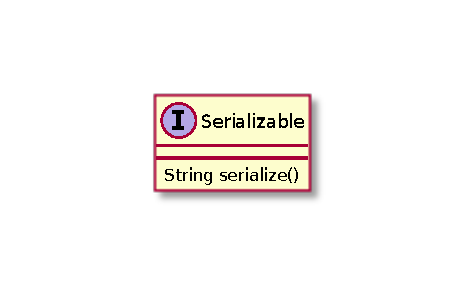
\includegraphics[width=\textwidth]{packageDiagrams/serializationPackage}
\end{figure}


\subsubsection{Class \texttt{SerializationUtilities}}
\label{type:edu.kit.wavelength.client.model.serialization.SerializationUtilities}
Static class that provides tools for serializing and deserializing aggregate
 data.

Static methods:
\begin{itemize}
\item \texttt{List<String> extract(String input)}

Deserializes a string that was produced by the enclose method into its
 components.

\texttt{input}: The serialized string

Returns: The components that were serialized

\item \texttt{StringBuilder enclose(StringBuilder[] content)}

Creates a compound serialized string from a set of serialized strings that
 can be deserialized with extract.

\texttt{content}: The components

Returns: A string that is a serializations of all component strings

\item \texttt{<T> List<T> deserializeList(String serialized, Function<String, T> deserialize)}

Deserializes a list created by serializeList.

\texttt{serialized}: The serialization string created by serializeList

\texttt{deserialize}: The deserialization method for a single list element

Returns: A list of deserialized elements

\item \texttt{<T> StringBuilder serializeList(List<T> list, Function<T, StringBuilder> serialize)}

Serializes a list of elements of the same type.

\texttt{list}: The list of elements

\texttt{serialize}: The serialize method for a single element

Returns: A serialization string for the entire list

\end{itemize}

\subsubsection{Interface \texttt{Serializable}}
\label{type:edu.kit.wavelength.client.model.serialization.Serializable}
Implemented by objects that may be serialized into a string.

Methods:
\begin{itemize}
\item \texttt{StringBuilder serialize()}

Creates a string designating the object's state.

Returns: A string designating the object's state from which it can be restored
         using a corresponding deserialization method

\end{itemize}

\subsection{Package \lstinline{edu.kit.wavelength.client.model.term}}
\label{pkg:edu.kit.wavelength.client.model.term}
The \texttt{term} package contains the classes used by the application to
represent lambda terms and provides means for operating on them.

Lambda terms are represented as a tree structure of immutable objects
implementing the interface \texttt{\lnk{LambdaTerm}}. There are four types that
directly model their corresponding entities in the untyped lambda calculus:
\texttt{\lnk{Abstraction}}, \texttt{\lnk{Application}}, \texttt{\lnk{BoundVariable}} and
\texttt{\lnk{FreeVariable}}. For abstractions, the preferred name for the variable is stored.
Bound variables refer to their corresponding abstraction using De Bruijn indices.
Additionally, there are two more types that do not have
a direct counterpart in untyped lambda calculus: \texttt{\lnk{NamedTerm}} and
\texttt{\lnk{PartialApplication}}.

\texttt{\lnk{NamedTerm}} is a lambda term that has been assigned a name, either by a
library or by the user. In some cases (for instance when considered by a
reduction order polcy) it should be treated exactly like the term it
represents. In other cases (for instance when displaying the term) it should be
treated differently.

\texttt{\lnk{PartialApplication}} represents a series of nested applications, with
the left hand side of the innermost application being a named term that stands
for a library function (which is a series of nested abstractions). An
application where the left hand side is a partial application can be
transformed into a larger partial application. When the partial application
has collected as many arguments as the library function its inner named
term represents, it will be evaluated in one step and replaced by a lambda
term for its result. The purpose of this is to be able to accelerate large
computations involving numbers.

Except for testing for equality, all operations on lambda terms are carried out
by visitors. In addition to the universal \texttt{\lnk{Visitor}<T>} interface, which
is implemented by visitors carrying out an operation and returning a result of type
\texttt{T}, there are several abstract classes implementing this interface to make
typical operations on lambda terms easier. \texttt{\lnk{NameAgnosticVisitor}<T>} is a
visitor that ignores the names of terms (such as reduction orders),
\texttt{\lnk{ResolvedNamesVisitor}<T>} provides non-colliding names for variable names
used in abstractions and is intended for visitors displaying lambda terms, and
\texttt{\lnk{TermTransformer}} allows transforming a lambda term into a new term while
automatically removing the name tag from lambda terms that have been changed by
the transformation. It is intended for substitution operations and $\beta$-reductions.

\begin{figure}[H]
	\centering
	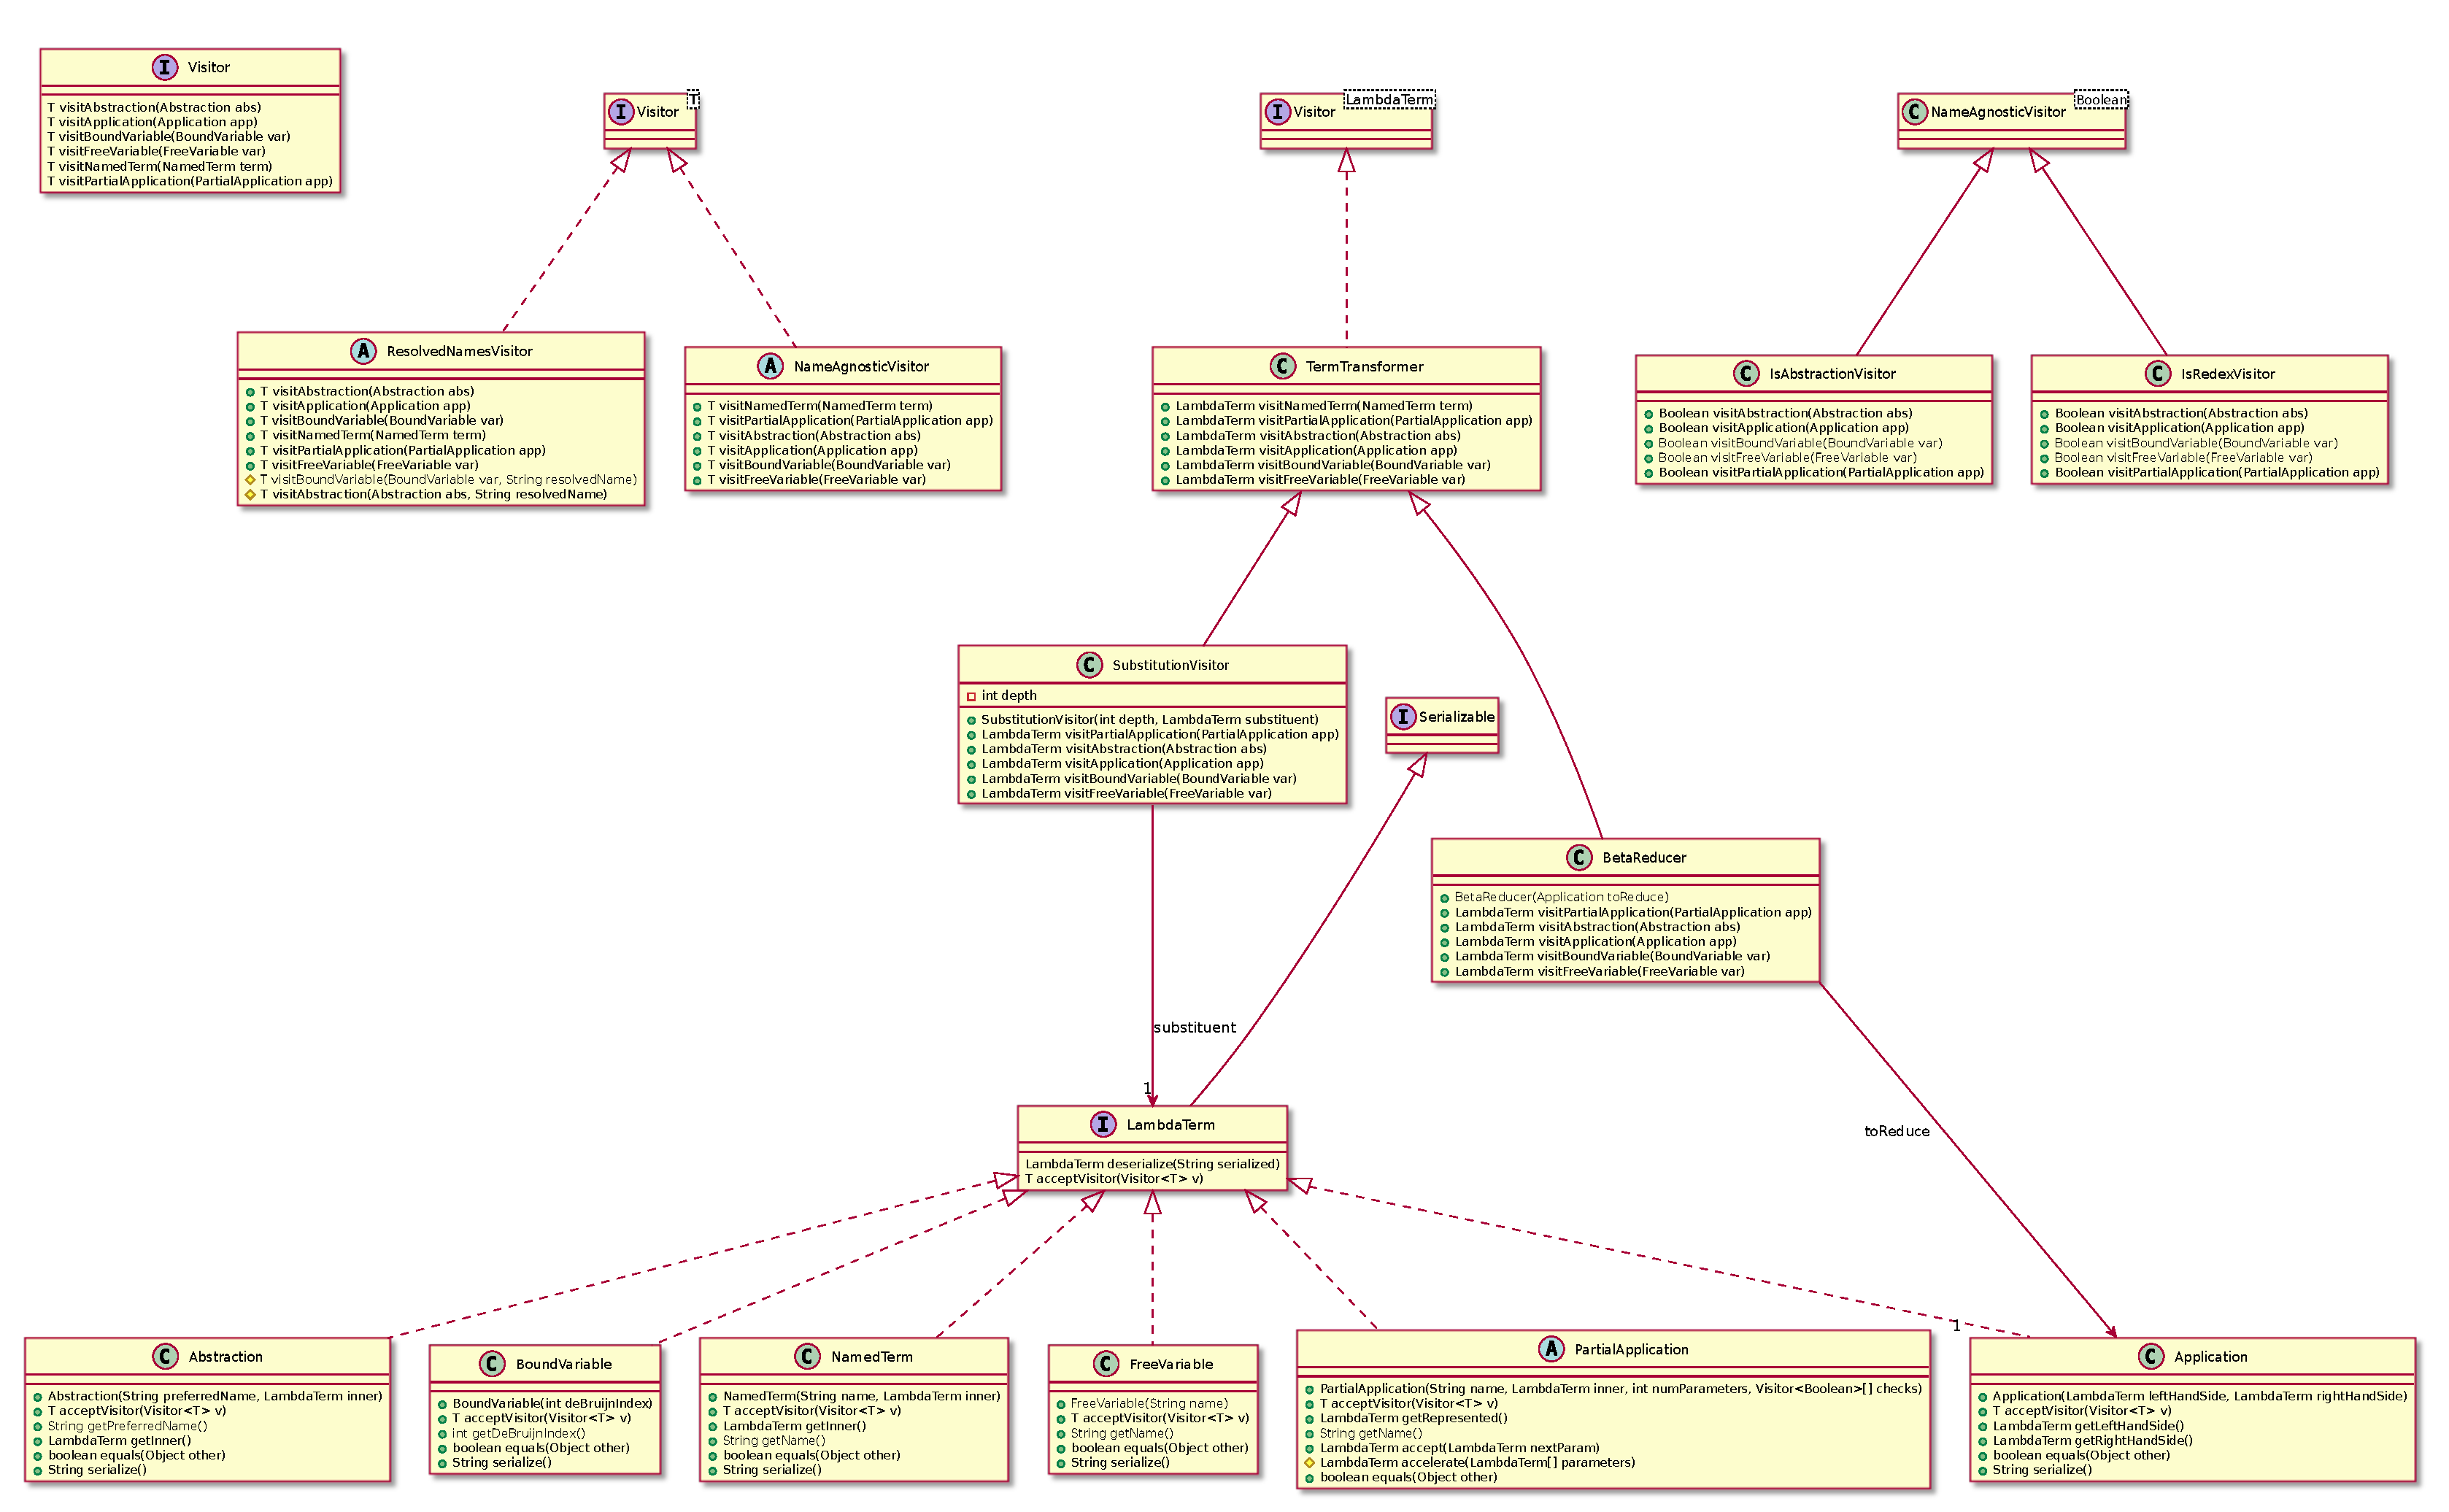
\includegraphics[width=\textwidth]{packageDiagrams/termPackage}
\end{figure}

\subsubsection{Interface \texttt{Visitor<T>}}
\label{type:edu.kit.wavelength.client.model.term.Visitor}
Represents a visitor that visits \texttt{lambdaTerm}s and returns objects of a
 given type upon visiting a \texttt{lambdaTerm}.

\texttt{<T>}: The type of object that is returned when visiting a term.

Methods:
\begin{itemize}
\item \texttt{T visitAbstraction(\hyperref[type:edu.kit.wavelength.client.model.term.Abstraction]{Abstraction} abs)}

Visit an \texttt{Abstraction}.

\texttt{abs}: The \texttt{Abstraction} to be visited

Returns: The return value of the \texttt{Visitor} when visiting the given
         \texttt{Abstraction}

\item \texttt{T visitApplication(\hyperref[type:edu.kit.wavelength.client.model.term.Application]{Application} app)}

Visit an \texttt{Application}.

\texttt{app}: The \texttt{Application} to be visited

Returns: The return value of the \texttt{Visitor} when visiting the given
         \texttt{Application}

\item \texttt{T visitBoundVariable(\hyperref[type:edu.kit.wavelength.client.model.term.BoundVariable]{BoundVariable} var)}

Visit a \texttt{BoundVariable}.

\texttt{var}: The \texttt{BoundVariable} to be visited

Returns: The return value of the \texttt{Visitor} when visiting the given
         \texttt{BoundVariable}

\item \texttt{T visitFreeVariable(\hyperref[type:edu.kit.wavelength.client.model.term.FreeVariable]{FreeVariable} var)}

Visit a \texttt{FreeVariable}.

\texttt{var}: The \texttt{FreeVariable} to be visited

Returns: The return value of the \texttt{Visitor} when visiting the given
         \texttt{FreeVariable}

\item \texttt{T visitNamedTerm(\hyperref[type:edu.kit.wavelength.client.model.term.NamedTerm]{NamedTerm} term)}

Visit a \texttt{NamedTerm}.

\texttt{term}: The \texttt{NamedTerm} to be visited

Returns: The return value of the \texttt{Visitor} when visiting the given
         \texttt{NamedTerm}

\item \texttt{T visitPartialApplication(\hyperref[type:edu.kit.wavelength.client.model.term.PartialApplication]{PartialApplication} app)}

Visit a \texttt{PartialApplication}.

\texttt{app}: The \texttt{PartialApplication} to be visited

Returns: The return value of the \texttt{Visitor} when visiting the given
         \texttt{PartialApplication}

\end{itemize}

\subsubsection{Abstract Class \texttt{TermTransformer}}
\label{type:edu.kit.wavelength.client.model.term.TermTransformer}
Implements: \texttt{\hyperref[type:edu.kit.wavelength.client.model.term.Visitor]{Visitor}}

A \texttt{Visitor} that performs a transformation of some kind of a
 \texttt{LambdaTerm}, automatically removing names if their inner term has been
 changed by the transformation.

\subsubsection{Class \texttt{SubstitutionVisitor}}
\label{type:edu.kit.wavelength.client.model.term.SubstitutionVisitor}
Extends: \texttt{\hyperref[type:edu.kit.wavelength.client.model.term.TermTransformer]{TermTransformer}}

A \texttt{Visitor} that substitutes \texttt{BoundVariable}s with a given De
 Bruijn index with a given substituent.

Constructors:
\begin{itemize}
\item \texttt{SubstitutionVisitor(\hyperref[type:edu.kit.wavelength.client.model.term.LambdaTerm]{LambdaTerm} substituent)}

Creates a new substitution visitor.

\texttt{substituent}: The term that should be substituted with

\end{itemize}

\subsubsection{Abstract Class \texttt{ResolvedNamesVisitor<T>}}
\label{type:edu.kit.wavelength.client.model.term.ResolvedNamesVisitor}
Implements: \texttt{\hyperref[type:edu.kit.wavelength.client.model.term.Visitor]{Visitor}}

A \texttt{Visitor} that gives non-colliding names for bound variables.

\texttt{<T>}: The return value of the visitor

Constructors:
\begin{itemize}
\item \texttt{ResolvedNamesVisitor(List<\hyperref[type:edu.kit.wavelength.client.model.library.Library]{Library}> libraries)}

Creates a new ResolvedNamesVisitor that checks the given libraries for names
 that should not be emitted.

\texttt{libraries}: The libraries that are assumed in the ambient context of the terms
            being visited

\end{itemize}

Methods:
\begin{itemize}
\item \texttt{protected abstract T visitBoundVariable(\hyperref[type:edu.kit.wavelength.client.model.term.BoundVariable]{BoundVariable} var, String resolvedName)}

Visit a \texttt{BoundVariable} with an additional non-colliding name for said
 variable.
 
 This method is provided merely for convenience, the given name will be the
 same as the one provided for the given abstraction.

\texttt{var}: The \texttt{BoundVariable} to be visited

\texttt{resolvedName}: The resolved name for the \texttt{BoundVariable}

Returns: The return value of the \texttt{Visitor} upon visiting the given
         \texttt{BoundVariable}

\item \texttt{protected abstract T visitAbstraction(\hyperref[type:edu.kit.wavelength.client.model.term.Abstraction]{Abstraction} abs, String resolvedName)}

Visit an \texttt{Abstraction} with an additional non-colliding name for its
 variable.

\texttt{abs}: The \texttt{Abstraction} to be visited

\texttt{resolvedName}: The resolved name for the variable of this \texttt{Abstraction}

Returns: The return value of the visitor upon visiting the given
         \texttt{Abstraction}

\end{itemize}

\subsubsection{Abstract Class \texttt{PartialApplication}}
\label{type:edu.kit.wavelength.client.model.term.PartialApplication}
Implements: \texttt{\hyperref[type:edu.kit.wavelength.client.model.term.LambdaTerm]{LambdaTerm}}

Represents a \texttt{LambdaTerm} that consists of a library function that may
 be accelerated, as well as zero or more applications with arguments for said
 library function.

Constructors:
\begin{itemize}
\item \texttt{protected PartialApplication(String name, \hyperref[type:edu.kit.wavelength.client.model.term.LambdaTerm]{LambdaTerm} inner, int numParameters, List<\hyperref[type:edu.kit.wavelength.client.model.term.Visitor]{Visitor}<Boolean>> checks)}

Creates a new partial application that has not yet bound any parameters.

\texttt{name}: The name of the library function.

\texttt{inner}: The \texttt{LambdaTerm} for the non-accelerated library function

\texttt{numParameters}: The number of parameters that the library function takes

\texttt{checks}: For each parameter, a \texttt{Visitor} that checks whether the
            given parameter has the correct format for acceleration

\end{itemize}

Methods:
\begin{itemize}
\item \texttt{\hyperref[type:edu.kit.wavelength.client.model.term.LambdaTerm]{LambdaTerm}[] getReceived()}

Returns the array of received terms.

Returns: An array of received terms. Only the first getNumReceived elements
         are valid.

\item \texttt{int getNumReceived()}

Returns the number of received terms.

Returns: The number of received terms

\item \texttt{\hyperref[type:edu.kit.wavelength.client.model.term.LambdaTerm]{LambdaTerm} getRepresented()}

Returns the \texttt{LambdaTerm} that this partial application represents.

Returns: The \texttt{LambdaTerm} that this partial application represents

\item \texttt{String getName()}



\item \texttt{\hyperref[type:edu.kit.wavelength.client.model.term.LambdaTerm]{LambdaTerm} accept(\hyperref[type:edu.kit.wavelength.client.model.term.LambdaTerm]{LambdaTerm} nextParam)}

Accepts a new parameter for the partial application.
 
 If the parameter does not match the format that can be accelerated, returns a
 new term representing the unaccelerated application.
 
 If the parameter matches the format that can be accelerated, returns the
 result of the operation represented by the partial application if all
 parameters are now present, or a new PartialApplication representing the
 partial application including the given parameter.

\texttt{nextParam}: The parameter to be accepted

Returns: A \texttt{LambdaTerm} for the partial application with the new
         parameter as described above

\item \texttt{protected abstract \hyperref[type:edu.kit.wavelength.client.model.term.LambdaTerm]{LambdaTerm} accelerate(\hyperref[type:edu.kit.wavelength.client.model.term.LambdaTerm]{LambdaTerm}[] parameters)}

Directly determine the result of the computation given all parameters.

\texttt{parameters}: The parameters for the computation

Returns: The result of the computation

\item \texttt{protected void absorbClone(\hyperref[type:edu.kit.wavelength.client.model.term.PartialApplication]{PartialApplication} other)}



\item \texttt{protected StringBuilder serializeReceived()}



\item \texttt{protected void deserializeReceived(String serialized)}



\end{itemize}

\subsubsection{Class \texttt{PartialApplication.Addition}}
\label{type:edu.kit.wavelength.client.model.term.PartialApplication.Addition}
Extends: \texttt{\hyperref[type:edu.kit.wavelength.client.model.term.PartialApplication]{PartialApplication}}

Represents an acceleratable addition of church numbers.

Constructors:
\begin{itemize}
\item \texttt{Addition()}

Creates a new addition.

\end{itemize}

Static methods:
\begin{itemize}
\item \texttt{\hyperref[type:edu.kit.wavelength.client.model.term.PartialApplication.Addition]{PartialApplication.Addition} fromSerialized(String serialized)}

Restores a serialized addition.

\texttt{serialized}: The serialized addition

Returns: The restored addition

\end{itemize}

\subsubsection{Class \texttt{PartialApplication.Successor}}
\label{type:edu.kit.wavelength.client.model.term.PartialApplication.Successor}
Extends: \texttt{\hyperref[type:edu.kit.wavelength.client.model.term.PartialApplication]{PartialApplication}}

Represents the acceleratable successor operation on church numbers.

Constructors:
\begin{itemize}
\item \texttt{Successor()}

Creates a new successor operation

\end{itemize}

Static methods:
\begin{itemize}
\item \texttt{\hyperref[type:edu.kit.wavelength.client.model.term.PartialApplication.Successor]{PartialApplication.Successor} fromSerialized(String serialized)}

Restores a serialized successor operation.

\texttt{serialized}: The serialized successor

Returns: The restored succor

\end{itemize}

\subsubsection{Class \texttt{PartialApplication.Multiplication}}
\label{type:edu.kit.wavelength.client.model.term.PartialApplication.Multiplication}
Extends: \texttt{\hyperref[type:edu.kit.wavelength.client.model.term.PartialApplication]{PartialApplication}}

An acceleratable multiplication operation.

Constructors:
\begin{itemize}
\item \texttt{Multiplication()}

Creates a new instance of the multiplication operation.

\end{itemize}

Static methods:
\begin{itemize}
\item \texttt{\hyperref[type:edu.kit.wavelength.client.model.term.PartialApplication.Multiplication]{PartialApplication.Multiplication} fromSerialized(String serialized)}

Restores a serialized multiplication operation.

\texttt{serialized}: A serialized multiplication operation

Returns: The restored multiplication

\end{itemize}

\subsubsection{Class \texttt{PartialApplication.Exponentiation}}
\label{type:edu.kit.wavelength.client.model.term.PartialApplication.Exponentiation}
Extends: \texttt{\hyperref[type:edu.kit.wavelength.client.model.term.PartialApplication]{PartialApplication}}

An acceleratable exponentitation operation.

Constructors:
\begin{itemize}
\item \texttt{Exponentiation()}

Creates a new instance of the exponentiation operation.

\end{itemize}

Static methods:
\begin{itemize}
\item \texttt{\hyperref[type:edu.kit.wavelength.client.model.term.PartialApplication.Exponentiation]{PartialApplication.Exponentiation} fromSerialized(String serialized)}

Restores a serialized exponentiation.

\texttt{serialized}: The serialized exponentiation

Returns: The restored exponentiation

\end{itemize}

\subsubsection{Class \texttt{PartialApplication.Predecessor}}
\label{type:edu.kit.wavelength.client.model.term.PartialApplication.Predecessor}
Extends: \texttt{\hyperref[type:edu.kit.wavelength.client.model.term.PartialApplication]{PartialApplication}}

An acceleratable predecessor operation.

Constructors:
\begin{itemize}
\item \texttt{Predecessor()}

Creates a new predecessor operation.

\end{itemize}

Static methods:
\begin{itemize}
\item \texttt{\hyperref[type:edu.kit.wavelength.client.model.term.PartialApplication.Predecessor]{PartialApplication.Predecessor} fromSerialized(String serialized)}

Restores a serialized predecessor operation.

\texttt{serialized}: The serialized predecessor operation

Returns: The restored predecessor operation

\end{itemize}

\subsubsection{Class \texttt{PartialApplication.Subtraction}}
\label{type:edu.kit.wavelength.client.model.term.PartialApplication.Subtraction}
Extends: \texttt{\hyperref[type:edu.kit.wavelength.client.model.term.PartialApplication]{PartialApplication}}

Represents an acceleratable subtraction operation.

Constructors:
\begin{itemize}
\item \texttt{Subtraction()}

Creates a new subtraction operation.

\end{itemize}

Static methods:
\begin{itemize}
\item \texttt{\hyperref[type:edu.kit.wavelength.client.model.term.PartialApplication.Subtraction]{PartialApplication.Subtraction} fromSerialized(String serialized)}

Restores a subtraction operation from its serialization.

\texttt{serialized}: The serialized subtraction

Returns: The restored subtraction

\end{itemize}

\subsubsection{Class \texttt{NamedTerm}}
\label{type:edu.kit.wavelength.client.model.term.NamedTerm}
Implements: \texttt{\hyperref[type:edu.kit.wavelength.client.model.term.LambdaTerm]{LambdaTerm}}

Represents a \texttt{LambdaTerm} that has a name.

Constructors:
\begin{itemize}
\item \texttt{NamedTerm(String name, \hyperref[type:edu.kit.wavelength.client.model.term.LambdaTerm]{LambdaTerm} inner)}

Creates a new named term.

\texttt{name}: The name of the term

\texttt{inner}: The actual term that is being named

\end{itemize}

Static methods:
\begin{itemize}
\item \texttt{\hyperref[type:edu.kit.wavelength.client.model.term.NamedTerm]{NamedTerm} fromSerialized(String serialized)}

Restores a serialized named term.

\texttt{serialized}: The serialization of a named term

Returns: The restored named term

\end{itemize}

Methods:
\begin{itemize}
\item \texttt{\hyperref[type:edu.kit.wavelength.client.model.term.LambdaTerm]{LambdaTerm} getInner()}

Returns the term that the named term represents.

Returns: The term that the named term represents

\item \texttt{String getName()}

Returns the name of the term.

Returns: The name of the term

\end{itemize}

\subsubsection{Abstract Class \texttt{NameAgnosticVisitor<T>}}
\label{type:edu.kit.wavelength.client.model.term.NameAgnosticVisitor}
Implements: \texttt{\hyperref[type:edu.kit.wavelength.client.model.term.Visitor]{Visitor}}

A \texttt{Visitor} that will treat a \texttt{NamedTerm} precisely like the term
 that it represents.

\texttt{<T>}: The return value of the \texttt{Visitor}

\subsubsection{Interface \texttt{LambdaTerm}}
\label{type:edu.kit.wavelength.client.model.term.LambdaTerm}
Extends: \texttt{\hyperref[type:edu.kit.wavelength.client.model.serialization.Serializable]{Serializable}}

Represents a term in the untyped lambda calculus.

Static methods:
\begin{itemize}
\item \texttt{\hyperref[type:edu.kit.wavelength.client.model.term.LambdaTerm]{LambdaTerm} deserialize(String serialized)}

Creates a lambda term from its serialization.

\texttt{serialized}: The serialized representation of the lambda term

Returns: A lambda term that is equal to the term that was serialized

\item \texttt{\hyperref[type:edu.kit.wavelength.client.model.term.LambdaTerm]{LambdaTerm} churchNumber(int value)}

Returns a named lambda term that corresponds to a church number.

\texttt{value}: The value of the church number to construct

Returns: The requested church number

\end{itemize}

Methods:
\begin{itemize}
\item \texttt{\hyperref[type:edu.kit.wavelength.client.model.term.LambdaTerm]{LambdaTerm} clone()}

Creates a deep clone of the lambda term.

Returns: A deep clone

\item \texttt{<T> T acceptVisitor(\hyperref[type:edu.kit.wavelength.client.model.term.Visitor]{Visitor}<T> v)}

Accept a \texttt{Visitor} by invoking the correct visit* method.

\texttt{v}: The \texttt{Visitor} whose correct visit* method should be invoked

Returns: The return value of the invoked visit* method

\end{itemize}

\subsubsection{Class \texttt{IsRedexVisitor}}
\label{type:edu.kit.wavelength.client.model.term.IsRedexVisitor}
Extends: \texttt{\hyperref[type:edu.kit.wavelength.client.model.term.NameAgnosticVisitor]{NameAgnosticVisitor}}

A \texttt{Visitor} that returns a boolean that is true if the given
 \texttt{LambdaTerm} represents a redex (possibly bound to one or more nested
 names).

\subsubsection{Class \texttt{IsPartialApplicationVisitor}}
\label{type:edu.kit.wavelength.client.model.term.IsPartialApplicationVisitor}
Extends: \texttt{\hyperref[type:edu.kit.wavelength.client.model.term.NameAgnosticVisitor]{NameAgnosticVisitor}}

A visitor that returns true iff it was invoked on a partial application.

\subsubsection{Class \texttt{IsChurchNumberVisitor}}
\label{type:edu.kit.wavelength.client.model.term.IsChurchNumberVisitor}
Extends: \texttt{\hyperref[type:edu.kit.wavelength.client.model.term.NameAgnosticVisitor]{NameAgnosticVisitor}}



Constructors:
\begin{itemize}
\item \texttt{IsChurchNumberVisitor(int abstractionsSeen)}



\end{itemize}

\subsubsection{Class \texttt{IsAbstractionVisitor}}
\label{type:edu.kit.wavelength.client.model.term.IsAbstractionVisitor}
Extends: \texttt{\hyperref[type:edu.kit.wavelength.client.model.term.NameAgnosticVisitor]{NameAgnosticVisitor}}

A \texttt{Visitor} that returns a boolean that is true if and only if the
 given \texttt{LambdaTerm} represents an \texttt{Abstraction} (possibly bound to
 one or more nested names).

\subsubsection{Class \texttt{GetChurchNumberVisitor}}
\label{type:edu.kit.wavelength.client.model.term.GetChurchNumberVisitor}
Extends: \texttt{\hyperref[type:edu.kit.wavelength.client.model.term.NameAgnosticVisitor]{NameAgnosticVisitor}}



\subsubsection{Class \texttt{FreeVariable}}
\label{type:edu.kit.wavelength.client.model.term.FreeVariable}
Implements: \texttt{\hyperref[type:edu.kit.wavelength.client.model.term.LambdaTerm]{LambdaTerm}}

Represents a free variable in the untyped lambda calculus.
 
 A free variable has a name. Unlike the name of the variable bound during an
 abstraction, this name is not a preferred name, but fixed, since it is free
 over the entire lambda term that is being represented. Changing this name
 would therefore change the lambda term.

Constructors:
\begin{itemize}
\item \texttt{FreeVariable(String name)}

Creates a new free variable term.

\texttt{name}: The name of the free variable being referenced

\end{itemize}

Static methods:
\begin{itemize}
\item \texttt{\hyperref[type:edu.kit.wavelength.client.model.term.FreeVariable]{FreeVariable} fromSerialized(String serialized)}

Restores a free variable from its serialization.

\texttt{serialized}: A serialized free variable

Returns: The free variable referred to by the serialization

\end{itemize}

Methods:
\begin{itemize}
\item \texttt{String getName()}

Returns the name of the free variable.

Returns: The name of the free variable

\end{itemize}

\subsubsection{Class \texttt{BoundVariable}}
\label{type:edu.kit.wavelength.client.model.term.BoundVariable}
Implements: \texttt{\hyperref[type:edu.kit.wavelength.client.model.term.LambdaTerm]{LambdaTerm}}

Represents a bound variable in the untyped lambda calculus.
 
 It refers to its corresponding \texttt{Abstraction} using its De Bruijn index.

Constructors:
\begin{itemize}
\item \texttt{BoundVariable(int deBruijnIndex)}

Creates a new bound variable term.

\texttt{deBruijnIndex}: The De Bruijn index of the term

\end{itemize}

Static methods:
\begin{itemize}
\item \texttt{\hyperref[type:edu.kit.wavelength.client.model.term.BoundVariable]{BoundVariable} fromSerialized(String serialized)}

Restores a bound variable from its serialization.

\texttt{serialized}: A serialized bound variable

Returns: The bound variable that the serialization string describes

\end{itemize}

Methods:
\begin{itemize}
\item \texttt{int getDeBruijnIndex()}

Returns the De Bruijn index of the variable.

Returns: The De Bruijn index

\end{itemize}

\subsubsection{Class \texttt{BetaReducer}}
\label{type:edu.kit.wavelength.client.model.term.BetaReducer}
Extends: \texttt{\hyperref[type:edu.kit.wavelength.client.model.term.TermTransformer]{TermTransformer}}

A \texttt{Visitor} that transforms a \texttt{LambdaTerm} by beta reducing a
 given redex.

Constructors:
\begin{itemize}
\item \texttt{BetaReducer(\hyperref[type:edu.kit.wavelength.client.model.term.Application]{Application} toReduce)}

Creates a new beta reducer that reduces the given redex.

\texttt{toReduce}: The application that should be reduced. This must be a redex,
            otherwise an exception is thrown.

\end{itemize}

\subsubsection{Class \texttt{Application}}
\label{type:edu.kit.wavelength.client.model.term.Application}
Implements: \texttt{\hyperref[type:edu.kit.wavelength.client.model.term.LambdaTerm]{LambdaTerm}}

Represents an application in the untyped lambda calculus.
 
 An application has a left hand side and a right hand side, both of which may
 be arbitrary lambda terms.

Constructors:
\begin{itemize}
\item \texttt{Application(\hyperref[type:edu.kit.wavelength.client.model.term.LambdaTerm]{LambdaTerm} leftHandSide, \hyperref[type:edu.kit.wavelength.client.model.term.LambdaTerm]{LambdaTerm} rightHandSide)}

Creates a new application.

\texttt{leftHandSide}: The left hand side of the application

\texttt{rightHandSide}: The right hand side of the application

\end{itemize}

Static methods:
\begin{itemize}
\item \texttt{\hyperref[type:edu.kit.wavelength.client.model.term.Application]{Application} fromSerialized(String serialized)}

Restores an application from its serialization.

\texttt{serialized}: A serialized application

Returns: The restored application

\end{itemize}

Methods:
\begin{itemize}
\item \texttt{\hyperref[type:edu.kit.wavelength.client.model.term.LambdaTerm]{LambdaTerm} getLeftHandSide()}

Returns the left hand side of the application.

Returns: The left hand side of the application

\item \texttt{\hyperref[type:edu.kit.wavelength.client.model.term.LambdaTerm]{LambdaTerm} getRightHandSide()}

Returns the right hand side of the application.

Returns: The right hand side of the application

\end{itemize}

\subsubsection{Class \texttt{Abstraction}}
\label{type:edu.kit.wavelength.client.model.term.Abstraction}
Implements: \texttt{\hyperref[type:edu.kit.wavelength.client.model.term.LambdaTerm]{LambdaTerm}}

Represents an abstraction in the untyped lambda calculus.
 
 An abstraction has an inner term and a preferred name for the variable it
 abstracts. When displaying the abstraction, a different name may be used,
 since terms referring to this abstraction will use De Bruijn indices to do
 so.

Constructors:
\begin{itemize}
\item \texttt{Abstraction(String preferredName, \hyperref[type:edu.kit.wavelength.client.model.term.LambdaTerm]{LambdaTerm} inner)}

Creates a new abstraction.

\texttt{preferredName}: The preferred name for the variable that is abstracted

\texttt{inner}: The lambda term that the abstraction encloses

\end{itemize}

Static methods:
\begin{itemize}
\item \texttt{\hyperref[type:edu.kit.wavelength.client.model.term.Abstraction]{Abstraction} fromSerialized(String serialized)}

Restores an abstraction from its serialization.

\texttt{serialized}: A serialized abstraction

Returns: The abstraction described by the serialization

\end{itemize}

Methods:
\begin{itemize}
\item \texttt{String getPreferredName()}

Gets the preferred name for the abstracted variable.

Returns: The preferred name

\item \texttt{\hyperref[type:edu.kit.wavelength.client.model.term.LambdaTerm]{LambdaTerm} getInner()}

Gets the inner term of the abstraction.

Returns: The term that this abstraction encloses

\end{itemize}

\subsection{Package \lstinline{edu.kit.wavelength.client.model.term.parsing}}
\label{pkg:edu.kit.wavelength.client.model.term.parsing}
Overview of \texttt{\pkg} with UML diagram.


\subsubsection{Class \texttt{Tokeniser}}
\label{type:edu.kit.wavelength.client.model.term.parsing.Tokeniser}
The Tokeniser class is used during the first step of the parsing process to
 turn the entered input into a sequence of Tokens.

Methods:
\begin{itemize}
\item \texttt{\hyperref[type:edu.kit.wavelength.client.model.term.parsing.Token]{Token}[] tokenise(String input, int offset, int rowPos)}

Divides a sequence of characters into Tokens.

\texttt{input}: The String to divide into tokens

Returns: An array containing all tokens

\end{itemize}

\subsubsection{Class \texttt{Token}}
\label{type:edu.kit.wavelength.client.model.term.parsing.Token}
Token objects are used by both the \texttt{Tokeniser} and the \texttt{Parser}
 during the construction of an \texttt{LambdaTerm} from an input String. Each
 token contains a part of the input String which can be accessed through this
 class' interface.

Constructors:
\begin{itemize}
\item \texttt{Token(String content, \hyperref[type:edu.kit.wavelength.client.model.term.parsing.TokenType]{TokenType} type, int start, int end)}

Creates a new Token containing the entered String and type.

\texttt{content}: The String to be stored in the Token

\texttt{type}: The Token's type

\end{itemize}

Methods:
\begin{itemize}
\item \texttt{String getContent()}

Used to access the String that makes up the token.

Returns: The String making up the token

\item \texttt{\hyperref[type:edu.kit.wavelength.client.model.term.parsing.TokenType]{TokenType} getType()}

Returns the type of the token.

Returns: The type of the token

\item \texttt{int getStart()}

Returns the start of the token.

Returns: The start of the token

\item \texttt{int getEnd()}

Returns the end of the token.

Returns: The end of the token

\end{itemize}

\subsubsection{Class \texttt{Parser}}
\label{type:edu.kit.wavelength.client.model.term.parsing.Parser}
This class is used to convert an input String into a \texttt{LambdaTerm}
 object. If any \texttt{Libraries} terms are used in the input, the necessary
 \texttt{Libraries} have to be passed to the Parser through its constructor.

Constructors:
\begin{itemize}
\item \texttt{Parser(List<\hyperref[type:edu.kit.wavelength.client.model.library.Library]{Library}> libraries)}

Initializes a new parser.

\texttt{libraries}: The \texttt{Libraries} to be taken into consideration during
            parsing

\end{itemize}

Methods:
\begin{itemize}
\item \texttt{\hyperref[type:edu.kit.wavelength.client.model.library.Library]{Library} getInputLibary()}

Gets a library containing the lambda terms and corresponding names defined in
 the the last invocation of \texttt{#parse(String)}}'s input String.

Returns: A \texttt{Library} containing the terms entered by the user with their
         assigned names

\item \texttt{\hyperref[type:edu.kit.wavelength.client.model.term.LambdaTerm]{LambdaTerm} parse(String input)}

Parses the input text representation of a lambda term and turns it into a
 \texttt{LambdaTerm} object if successful.

\texttt{input}: The String to parse.

Returns: The parsed \texttt{LambdaTerm} object

\end{itemize}

\subsubsection{Class \texttt{ParseException}}
\label{type:edu.kit.wavelength.client.model.term.parsing.ParseException}
Extends: \texttt{Exception}

An exception used to indicate an error during the parsing of an entered
 \texttt{LambdaTerm}.

Constructors:
\begin{itemize}
\item \texttt{ParseException(String message, int row, int columnStart, int columnEnd)}

Creates a new ParseException with the entered parameters.

\texttt{message}: A message to the user describing the error causing the exception

\texttt{row}: The row containing the source of this exception

\texttt{column}: The row containing the source of this exception

\end{itemize}

Methods:
\begin{itemize}
\item \texttt{int getRow()}

Gets the row in which the error causing this exception occurred.

Returns: The row in which the error occurred

\item \texttt{int getColumnStart()}

Gets the start column of the token in which the error causing this exception
 occurred.

Returns: The start column of the token in which the error occurred

\item \texttt{int getColumnEnd()}

Gets the end column of the token in which the error causing this exception
 occurred.

Returns: The end column of the token in which the error occurred

\end{itemize}

\subsection{Package \lstinline{edu.kit.wavelength.client.view.action}}
\label{pkg:edu.kit.wavelength.client.view.action}
Overview of \texttt{\pkg} with UML diagram.

\begin{figure}[H]
	\centering
	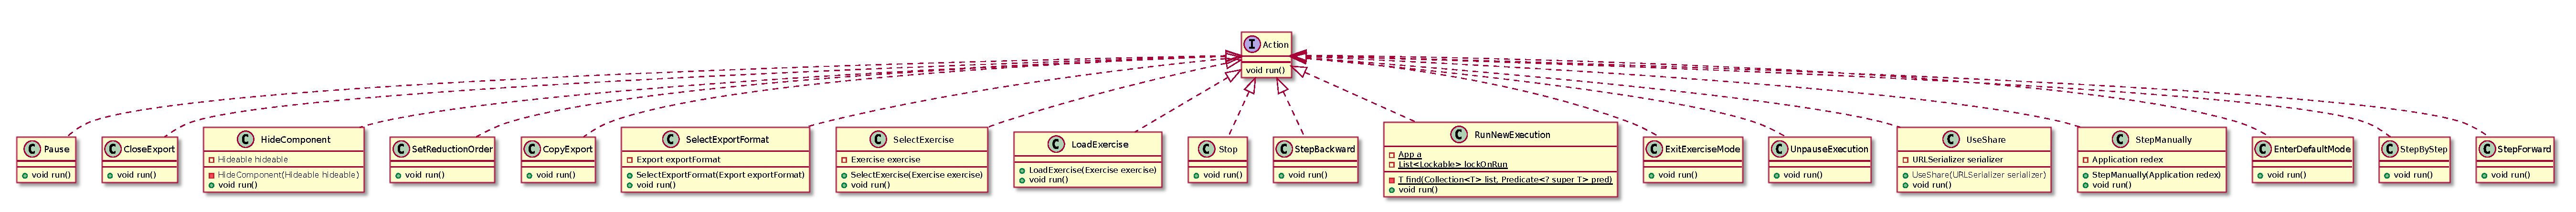
\includegraphics[width=\textwidth]{packageDiagrams/actionPackage}
\end{figure}


\subsubsection{Class \texttt{UseShare}}
\label{type:edu.kit.wavelength.client.view.action.UseShare}
Implements: \texttt{\hyperref[type:edu.kit.wavelength.client.view.action.Action]{Action}}

This action toggles the permalink panel. The permalink encodes the current
 input, output and settings.

Constructors:
\begin{itemize}
\item \texttt{UseShare(\hyperref[type:edu.kit.wavelength.client.view.URLSerializer]{URLSerializer} serializer)}

Constructs a new action handler for the permalink request.

\texttt{serializer}: The instance to delegate the serialization process to

\end{itemize}

Methods:
\begin{itemize}
\item \texttt{void run()}

Hides the share panel if it is currently shown, otherwise generates the
 permalink that encodes the current input, output and settings.

\end{itemize}

\subsubsection{Class \texttt{UnpauseExecution}}
\label{type:edu.kit.wavelength.client.view.action.UnpauseExecution}
Implements: \texttt{\hyperref[type:edu.kit.wavelength.client.view.action.Action]{Action}}

This action continues the paused reduction process.

Methods:
\begin{itemize}
\item \texttt{void run()}

Continues the paused reduction process, disables the step-by-step buttons and
 the option menu.

\end{itemize}

\subsubsection{Class \texttt{Stop}}
\label{type:edu.kit.wavelength.client.view.action.Stop}
Implements: \texttt{\hyperref[type:edu.kit.wavelength.client.view.action.Action]{Action}}

This action stops the currently running reduction process and re-enables all
 input related components.

Methods:
\begin{itemize}
\item \texttt{void run()}

Re-enables the editor and all option menus and blocks all buttons except the
 run button. Does not clear the output view.

\end{itemize}

\subsubsection{Class \texttt{StepManually}}
\label{type:edu.kit.wavelength.client.view.action.StepManually}
Implements: \texttt{\hyperref[type:edu.kit.wavelength.client.view.action.Action]{Action}}

Action that initiates a manual step on a particular redex in an output view.

Constructors:
\begin{itemize}
\item \texttt{StepManually(\hyperref[type:edu.kit.wavelength.client.model.term.Application]{Application} redex)}

Creates the action with the redex to apply when the user clicks on a
 redex.

\texttt{redex}: The redex to apply

\end{itemize}

Methods:
\begin{itemize}
\item \texttt{void run()}

Delegates the step to the Executor.

\end{itemize}

\subsubsection{Class \texttt{StepForward}}
\label{type:edu.kit.wavelength.client.view.action.StepForward}
Implements: \texttt{\hyperref[type:edu.kit.wavelength.client.view.action.Action]{Action}}

This action requests and displays the next reduction step of the current
 execution.

Methods:
\begin{itemize}
\item \texttt{void run()}

Requests and displays the next reduction step.

\end{itemize}

\subsubsection{Class \texttt{StepByStep}}
\label{type:edu.kit.wavelength.client.view.action.StepByStep}
Implements: \texttt{\hyperref[type:edu.kit.wavelength.client.view.action.Action]{Action}}

This class starts a new reduction process by requesting only the first
 reduction step.

Methods:
\begin{itemize}
\item \texttt{void run()}

Reads the users input and all required options from the option menus and
 delegates the reduction process to the Executor. Disables the editor and some
 option menus and toggles the buttons accordingly.

\end{itemize}

\subsubsection{Class \texttt{StepBackward}}
\label{type:edu.kit.wavelength.client.view.action.StepBackward}
Implements: \texttt{\hyperref[type:edu.kit.wavelength.client.view.action.Action]{Action}}

This class removes the last shown reduction step from the output.

Methods:
\begin{itemize}
\item \texttt{void run()}

Removes the last shown step from the output.

\end{itemize}

\subsubsection{Class \texttt{SetReductionOrder}}
\label{type:edu.kit.wavelength.client.view.action.SetReductionOrder}
Implements: \texttt{\hyperref[type:edu.kit.wavelength.client.view.action.Action]{Action}}

This action changes the reduction order for the further execution.

Methods:
\begin{itemize}
\item \texttt{void run()}

Changes the reduction order to the selected one.

\end{itemize}

\subsubsection{Class \texttt{SelectExportFormat}}
\label{type:edu.kit.wavelength.client.view.action.SelectExportFormat}
Implements: \texttt{\hyperref[type:edu.kit.wavelength.client.view.action.Action]{Action}}

This action displays the currently displayed output in the selected export
 format in a pop up export window.

Constructors:
\begin{itemize}
\item \texttt{SelectExportFormat(\hyperref[type:edu.kit.wavelength.client.view.export.Export]{Export} exportFormat)}

Constructs a new action handler for the selection of an export format.

\texttt{exportFormat}: The export format the user chose

\end{itemize}

Methods:
\begin{itemize}
\item \texttt{void run()}

Gets the representation of the current output in the selected export format
 and writes it into the export output window. Displays this window and disables
 user interaction with all elements, except the export window.

\end{itemize}

\subsubsection{Class \texttt{SelectExercise}}
\label{type:edu.kit.wavelength.client.view.action.SelectExercise}
Implements: \texttt{\hyperref[type:edu.kit.wavelength.client.view.action.Action]{Action}}

This action will try to load a new exercise and alerts the user that the
 content of the Editor would be overwritten.

Constructors:
\begin{itemize}
\item \texttt{SelectExercise(\hyperref[type:edu.kit.wavelength.client.view.action.LoadExercise]{LoadExercise} loadExerciseAction, \hyperref[type:edu.kit.wavelength.client.view.exercise.Exercise]{Exercise} selected)}

Constructor.

\texttt{loadExerciseAction}: - action to run with selected exercise

\texttt{selected}: - exercise that is selected when this action fires

\end{itemize}

Methods:
\begin{itemize}
\item \texttt{void run()}

Opens a PopupWindow if the content of the editor would be overwritten.
 Allows the user to choose whether he wants to continue.
 Otherwise just loads the selected exercise.

\end{itemize}

\subsubsection{Class \texttt{RunNewExecution}}
\label{type:edu.kit.wavelength.client.view.action.RunNewExecution}
Implements: \texttt{\hyperref[type:edu.kit.wavelength.client.view.action.Action]{Action}}

This class starts a new reduction process and sets the view accordingly.

Methods:
\begin{itemize}
\item \texttt{void run()}

Reads the users input and all required options from the option menus and
 delegates the reduction process to the Executor. Disables the editor and
 option menus and toggles the play button.

\end{itemize}

\subsubsection{Class \texttt{Pause}}
\label{type:edu.kit.wavelength.client.view.action.Pause}
Implements: \texttt{\hyperref[type:edu.kit.wavelength.client.view.action.Action]{Action}}

This class pauses the currently running execution process and allows the user
 to now navigate through the reduction process himself.

Methods:
\begin{itemize}
\item \texttt{void run()}

Pause the running execution and enable the step-by-step buttons. Also allow
 output window interactions and enable the reduction order option.

\end{itemize}

\subsubsection{Class \texttt{LoadExercise}}
\label{type:edu.kit.wavelength.client.view.action.LoadExercise}
Implements: \texttt{\hyperref[type:edu.kit.wavelength.client.view.action.Action]{Action}}

This class changes the view from standard input to exercise view to display
 the selected exercise.

Methods:
\begin{itemize}
\item \texttt{void run()}

Reduces the editors width and displays the task in the enabled task view
 window. Also shows buttons for exiting this exercise view and for displaying
 the sample solution.

\item \texttt{\hyperref[type:edu.kit.wavelength.client.view.exercise.Exercise]{Exercise} getExercise()}



\item \texttt{void setExercise(\hyperref[type:edu.kit.wavelength.client.view.exercise.Exercise]{Exercise} exercise)}



\end{itemize}

\subsubsection{Class \texttt{EnterDefaultMode}}
\label{type:edu.kit.wavelength.client.view.action.EnterDefaultMode}
Implements: \texttt{\hyperref[type:edu.kit.wavelength.client.view.action.Action]{Action}}

This class changes the view from exercise mode view to standard input view.

Methods:
\begin{itemize}
\item \texttt{void run()}

Resizes the editor window to full width, hides the solution and task
 windows and hides the buttons for exiting and showing the solution.

\end{itemize}

\subsubsection{Class \texttt{Control}}
\label{type:edu.kit.wavelength.client.view.action.Control}


Static methods:
\begin{itemize}
\item \texttt{void updateStepControls()}



\end{itemize}

\subsubsection{Interface \texttt{Action}}
\label{type:edu.kit.wavelength.client.view.action.Action}
The Action interface encapsulates all events that can occur from the user
 interacting with the UI.
 
 An Action class is the event handler for one UI event. It is triggered by
 interacting with the dedicated UI element.

Methods:
\begin{itemize}
\item \texttt{void run()}

Called when the Action is triggered.

\end{itemize}

\subsection{Package \lstinline{edu.kit.wavelength.client.view}}
\label{pkg:edu.kit.wavelength.client.view}
Overview of \texttt{\pkg} with UML diagram.


\subsubsection{Class \texttt{URLSerializer}}
\label{type:edu.kit.wavelength.client.view.URLSerializer}
Serializes the application's state into an URL every N milliseconds where N
 is definded in the constructor as pollingDelayMS.

Constructors:
\begin{itemize}
\item \texttt{URLSerializer(List<\hyperref[type:edu.kit.wavelength.client.view.SerializationObserver]{SerializationObserver}> serializationOutputs, int pollingDelayMS)}

Creates a new serializer.

\texttt{serializationOutputs}: Observers to update with new serialized URL

\texttt{pollingDelayMS}: Delay between every serialization iteration. The serializable may
            change, so we poll it.

\end{itemize}

Methods:
\begin{itemize}
\item \texttt{void startPolling()}

Starts polling (serializing) the serializable.

\item \texttt{boolean serialize()}

Executes a serialization instantly if the executor is not running. Else does
 nothing.

Returns: whether the serializer will continue to poll after this call

\end{itemize}

\subsubsection{Interface \texttt{SerializationObserver}}
\label{type:edu.kit.wavelength.client.view.SerializationObserver}
Observer that receives updates containing the most recent id of a
 serialization.

Methods:
\begin{itemize}
\item \texttt{void updateSerialized(String id)}

Updates the observer.

\texttt{id}: identifier belonging to the most recent serialization

\end{itemize}

\subsubsection{Class \texttt{App}}
\label{type:edu.kit.wavelength.client.view.App}
Implements: \texttt{\hyperref[type:edu.kit.wavelength.client.model.serialization.Serializable]{Serializable}}

App is a singleton that initializes and holds the view.

Static methods:
\begin{itemize}
\item \texttt{\hyperref[type:edu.kit.wavelength.client.view.App]{App} get()}

Creates a new instance of App if there is none.
 Returns a singleton instance of App.

Returns: singleton instance of App

\item \texttt{void autoScroll()}



\end{itemize}

Methods:
\begin{itemize}
\item \texttt{StringBuilder serialize()}

Serializes the Application by returning a String from which the state of
 the application can be recreated.

 The String holds information about the \texttt{Executor}, the
 \texttt{Editor}, the \texttt{OptionBox}es and the selected \texttt{Library}s
 in this order.

Returns: the string representation of the application

\item \texttt{void deserialize(String content)}

Deserializes the Application with the given String.

 This includes \texttt{Executor}, the \texttt{Editor}, the
 \texttt{OptionBox}es and the selected \texttt{Library}s. It sets the
 application into step by step mode if the Executor holds terms and leaves
 the application in its initial state else.

\texttt{content}: the string representing the state of the application

\item \texttt{DockLayoutPanel mainPanel()}



\item \texttt{DropDown mainMenu()}



\item \texttt{Button openMainMenuButton()}



\item \texttt{DropDownMenu mainMenuPanel()}



\item \texttt{DropDownHeader mainMenuLibraryTitle()}



\item \texttt{List<CheckBox> libraryCheckBoxes()}



\item \texttt{Divider mainMenuDivider()}



\item \texttt{DropDownHeader mainMenuExerciseTitle()}



\item \texttt{List<AnchorListItem> exerciseButtons()}



\item \texttt{Modal loadExercisePopup()}



\item \texttt{ModalBody loadExercisePopupBody()}



\item \texttt{Label loadExercisePopupText()}



\item \texttt{ModalFooter loadExercisePopupFooter()}



\item \texttt{Button loadExercisePopupOkButton()}



\item \texttt{Button loadExercisePopupCancelButton()}



\item \texttt{Modal closeExercisePopup()}



\item \texttt{ModalBody closeExercisePopupBody()}



\item \texttt{Label closeExercisePopupText()}



\item \texttt{ModalFooter closeExercisePopupFooter()}



\item \texttt{Button closeExercisePopupOkButton()}



\item \texttt{Button closeExercisePopupCancelButton()}



\item \texttt{FlowPanel footerPanel()}



\item \texttt{SplitLayoutPanel ioPanel()}



\item \texttt{DockLayoutPanel inputPanel()}



\item \texttt{FlowPanel outputArea()}



\item \texttt{FlowPanel inputControlPanel()}



\item \texttt{SplitLayoutPanel editorExercisePanel()}



\item \texttt{FlowPanel exercisePanel()}



\item \texttt{FlowPanel exerciseHeaderPanel()}



\item \texttt{FlowPanel exerciseControlPanel()}



\item \texttt{Label exerciseDescriptionLabel()}



\item \texttt{Button toggleSolutionButton()}



\item \texttt{Button closeExerciseButton()}



\item \texttt{TextArea solutionArea()}



\item \texttt{SimplePanel editorPanel()}



\item \texttt{FlowPanel optionBarPanel()}



\item \texttt{ListBox outputFormatBox()}



\item \texttt{ListBox reductionOrderBox()}



\item \texttt{ListBox outputSizeBox()}



\item \texttt{FlowPanel controlPanel()}



\item \texttt{FlowPanel stepByStepControlPanel()}



\item \texttt{Button backwardsButton()}



\item \texttt{Button stepByStepButton()}



\item \texttt{Button forwardButton()}



\item \texttt{FlowPanel runControlPanel()}



\item \texttt{Button cancelButton()}



\item \texttt{Button runButton()}



\item \texttt{Button pauseButton()}



\item \texttt{Button unpauseButton()}



\item \texttt{ButtonGroup exportDropupGroup()}



\item \texttt{Button openExportMenuButton()}



\item \texttt{DropDownMenu exportMenu()}



\item \texttt{List<AnchorListItem> exportButtons()}



\item \texttt{Modal exportPopup()}



\item \texttt{ModalBody exportPopupBody()}



\item \texttt{TextArea exportArea()}



\item \texttt{ModalFooter exportPopupFooter()}



\item \texttt{Button exportPopupBodyOkButton()}



\item \texttt{ButtonGroup shareGroup()}



\item \texttt{TextBox sharePanel()}



\item \texttt{Button shareButton()}



\item \texttt{\hyperref[type:edu.kit.wavelength.client.view.gwt.MonacoEditor]{MonacoEditor} editor()}



\item \texttt{\hyperref[type:edu.kit.wavelength.client.view.execution.Executor]{Executor} executor()}



\item \texttt{boolean unicodeIsSet()}



\item \texttt{void setUnicode(boolean value)}



\item \texttt{boolean treeIsSet()}



\item \texttt{void setTree(boolean value)}



\item \texttt{FlowPanel outputBlocker()}



\end{itemize}

\subsection{Package \lstinline{edu.kit.wavelength.client.view.execution}}
\label{pkg:edu.kit.wavelength.client.view.execution}
Overview of \texttt{\pkg} with UML diagram.


\subsubsection{Class \texttt{Executor}}
\label{type:edu.kit.wavelength.client.view.execution.Executor}
Implements: \texttt{\hyperref[type:edu.kit.wavelength.client.model.serialization.Serializable]{Serializable}}

Concurrently reduces lambda terms.

Constructors:
\begin{itemize}
\item \texttt{Executor(List<\hyperref[type:edu.kit.wavelength.client.view.execution.ExecutionObserver]{ExecutionObserver}> executionObservers, List<\hyperref[type:edu.kit.wavelength.client.view.execution.ControlObserver]{ControlObserver}> controlObservers)}

Creates a new Executor.

\texttt{executionObservers}: Observers to update with reduced lambda terms

\texttt{controlObservers}: Observers to notify when executor reaches certain states

\end{itemize}

Methods:
\begin{itemize}
\item \texttt{void start(String input, \hyperref[type:edu.kit.wavelength.client.model.reduction.ReductionOrder]{ReductionOrder} order, \hyperref[type:edu.kit.wavelength.client.model.output.OutputSize]{OutputSize} size, List<\hyperref[type:edu.kit.wavelength.client.model.library.Library]{Library}> libraries)}

Starts the automatic execution of the input, parsing the term and then
 reducing it.

\texttt{input}: code to parse and reduce

\texttt{order}: order with which to reduce

\texttt{size}: which terms to push to observers

\texttt{libraries}: libraries to consider when parsing

\item \texttt{void pause()}

Pauses the automatic execution, transitioning into the step by step mode.

\item \texttt{void unpause()}

Unpauses the automatic execution, transitioning from step by step mode into
 automatic execution.

\item \texttt{void terminate()}

Terminates the step by step- and automatic execution.

\item \texttt{void stepByStep(String input, \hyperref[type:edu.kit.wavelength.client.model.reduction.ReductionOrder]{ReductionOrder} order, \hyperref[type:edu.kit.wavelength.client.model.output.OutputSize]{OutputSize} size, List<\hyperref[type:edu.kit.wavelength.client.model.library.Library]{Library}> libraries)}

Initiates the step by step execution, allowing the caller to choose the next
 step.

\texttt{input}: code to parse and execute

\texttt{order}: order with which to reduce

\texttt{size}: which terms to push to observers

\texttt{libraries}: libraries to consider when parsing

\item \texttt{void stepForward()}

Executes a single reduction of the current lambda term.

\item \texttt{void stepForward(\hyperref[type:edu.kit.wavelength.client.model.term.Application]{Application} redex)}

Executes a single reduction of the supplied redex.

\texttt{redex}: The redex to be evaluated. Must be a redex, otherwise an exception
            is thrown

\item \texttt{void stepBackward()}

Reverts to the previously output lambda term.

\item \texttt{void setReductionOrder(\hyperref[type:edu.kit.wavelength.client.model.reduction.ReductionOrder]{ReductionOrder} reduction)}

Changes the active reduction order to the entered one.

\texttt{reduction}: The new reduction order

\item \texttt{boolean canStepBackward()}

Checks whether stepBackward is possible.

Returns: whether stepBackward is possible

\item \texttt{boolean canStepForward()}

Checks whether stepForward is possible.

Returns: whether stepForward is possible

\item \texttt{boolean isPaused()}

Checks whether the engine is paused (true iff engine is not terminated and
 paused).

Returns: whether the engine is paused

\item \texttt{boolean isTerminated()}

Checks whether the engine is terminated.

Returns: whether the engine is terminated

\item \texttt{boolean isRunning()}

Checks whether the engine is running (true iff engine is not terminated and
 not paused).

Returns: whether the engine is running

\item \texttt{void wipe()}

Wipes the memory of the last execution.

\item \texttt{List<\hyperref[type:edu.kit.wavelength.client.model.term.LambdaTerm]{LambdaTerm}> getDisplayed()}

Returns the currently displayed lambda terms.

Returns: lt

\item \texttt{List<\hyperref[type:edu.kit.wavelength.client.model.library.Library]{Library}> getLibraries()}

Returns the libraries in use by the engine.

Returns: libraries

\item \texttt{StringBuilder serialize()}

Serializes the Executor by serializing its ExecutionEngine.

Returns: The Executor serialized String representation

\item \texttt{void deserialize(String serialization)}

Deserializes the Executor by deserializing its ExecutionEngine. Also loads
 the correct content into OutputArea.

\texttt{serialization}: serialized Executor

\end{itemize}

\subsubsection{Interface \texttt{ExecutionObserver}}
\label{type:edu.kit.wavelength.client.view.execution.ExecutionObserver}
Observer that receives reduced terms. Necessary because Executor is
 concurrent with UI.

Methods:
\begin{itemize}
\item \texttt{void pushTerm(\hyperref[type:edu.kit.wavelength.client.model.term.LambdaTerm]{LambdaTerm} t)}

Pushes the most recent displayed term.

\texttt{t}: the most recent term

\item \texttt{void removeLastTerm()}

Removes the last displayed term.

\item \texttt{void clear()}

Resets the observer.

\item \texttt{void reloadLastTerm()}

Reloads the last displayed term.

\end{itemize}

\subsubsection{Interface \texttt{ControlObserver}}
\label{type:edu.kit.wavelength.client.view.execution.ControlObserver}
Observer that is notified when the Executor executes certain state transitions.

Methods:
\begin{itemize}
\item \texttt{void finish()}

Called when the Executor finishes its execution, i.e. the last term is reduced.

\end{itemize}

\subsection{Package \lstinline{edu.kit.wavelength.client.view.exercise}}
\label{pkg:edu.kit.wavelength.client.view.exercise}
The \texttt{\pkglnk{view.exercise}} package contains the Application's exercise system:

The \lnk{Exercise} interface specifies that Exercises consist of a name, a task, a solution and (optional) predefined variables.
The \lnk{ConcreteExercise} class gives an implementation allowing for a simple generation of Exercises.
Note that Exercises use String representations of $\lambda$-Terms which must be transformed to \texttt{\hyperref[type:edu.kit.wavelength.client.model.term.LambdaTerm]} objects when used.

The \lnk{Exercises} class static has only one method which statically returns a list of all available Exercises.



\subsubsection{Class \texttt{Exercises}}
\label{type:edu.kit.wavelength.client.view.exercise.Exercises}
Static class giving access to all available exercises.

Static methods:
\begin{itemize}
\item \texttt{List<\hyperref[type:edu.kit.wavelength.client.view.exercise.Exercise]{Exercise}> all()}

Returns an unmodifiable list of all available exercises.

Returns: An unmodifiable list that contains exactly one instance of every
         available exercise

\end{itemize}

\subsubsection{Interface \texttt{Exercise}}
\label{type:edu.kit.wavelength.client.view.exercise.Exercise}
An exercise consists of a task specifying what the User is supposed to do and
 a solution specifying what the result should look like. Additionally
 exercises may provide a basis for a given task.

Methods:
\begin{itemize}
\item \texttt{String getName()}

Gets the name of the exercise.

Returns: The name of the exercise

\item \texttt{String getTask()}

Returns the explanation of the exercise.

Returns: The description of the task

\item \texttt{String getSolution()}

Returns the sample solution. Note that this may not be the only possible
 solution.

Returns: The solution of the exercise

\item \texttt{boolean hasPredefinitions()}

Returns whether this has predefined code or not.

Returns: \texttt{true} if this Exercise has predefined code

\item \texttt{String getPredefinitions()}

Returns initial definitions that are supposed to be of help for the User.
 Note that this may be empty.

Returns: The predefined code

\end{itemize}

\subsubsection{Class \texttt{ConcreteExercise}}
\label{type:edu.kit.wavelength.client.view.exercise.ConcreteExercise}
Implements: \texttt{\hyperref[type:edu.kit.wavelength.client.view.exercise.Exercise]{Exercise}}

This class is a concrete implementation of the \texttt{Exercise} interface.
 The needed method's return values are set in the constructor.

Constructors:
\begin{itemize}
\item \texttt{ConcreteExercise(String name, String task, String solution, String predefinitions)}

Creates a new Exercise.

\texttt{name}: - name of the exercise

\texttt{task}: - problem task to display

\texttt{solution}: - intended solution for the problem

\texttt{predefinitions}: - initial code to load into the editor

\end{itemize}

\subsection{Package \lstinline{edu.kit.wavelength.client.view.export}}
\label{pkg:edu.kit.wavelength.client.view.export}
Overview of \texttt{\pkg} with UML diagram.


\subsubsection{Class \texttt{UnicodeExport}}
\label{type:edu.kit.wavelength.client.view.export.UnicodeExport}
Implements: \texttt{\hyperref[type:edu.kit.wavelength.client.view.export.Export]{Export}}

This class translates the given lambda terms into text using a unicode lambda
 letter and a unicode arrow.

\subsubsection{Class \texttt{PlaintextExport}}
\label{type:edu.kit.wavelength.client.view.export.PlaintextExport}
Implements: \texttt{\hyperref[type:edu.kit.wavelength.client.view.export.Export]{Export}}

This class translates the given lambda terms into plain text. This especially
 means that the generated representation does not contain unicode symbols (if
 the user didn't define any terms or variable with unicode symbols).

\subsubsection{Class \texttt{LispExportVisitor}}
\label{type:edu.kit.wavelength.client.view.export.LispExportVisitor}
Extends: \texttt{\hyperref[type:edu.kit.wavelength.client.view.export.BasicExportVisitor]{BasicExportVisitor}}

This class is a visitor to translate a lambda term into a string using Lisp
 syntax. However it is not guaranteed that the generated representation is
 executable Lisp code.

Constructors:
\begin{itemize}
\item \texttt{LispExportVisitor(List<\hyperref[type:edu.kit.wavelength.client.model.library.Library]{Library}> libraries)}



\end{itemize}

\subsubsection{Class \texttt{LispExport}}
\label{type:edu.kit.wavelength.client.view.export.LispExport}
Implements: \texttt{\hyperref[type:edu.kit.wavelength.client.view.export.Export]{Export}}

This class translates the given lambda terms into Lisp code. Since it is only
 a syntactic translation, it is not guaranteed that the generated output is
 executable Lisp.

\subsubsection{Class \texttt{LaTeXExportVisitor}}
\label{type:edu.kit.wavelength.client.view.export.LaTeXExportVisitor}
Extends: \texttt{\hyperref[type:edu.kit.wavelength.client.view.export.BasicExportVisitor]{BasicExportVisitor}}

This class is a visitor to translate a lambda term into a string using
 LaTeX syntax.

Constructors:
\begin{itemize}
\item \texttt{LaTeXExportVisitor(List<\hyperref[type:edu.kit.wavelength.client.model.library.Library]{Library}> libraries)}



\end{itemize}

\subsubsection{Class \texttt{LatexExport}}
\label{type:edu.kit.wavelength.client.view.export.LatexExport}
Implements: \texttt{\hyperref[type:edu.kit.wavelength.client.view.export.Export]{Export}}

This class translates the given lambda terms into LaTeX code. The generated
 representation assumes math mode when being pasted into an existing LaTeX
 document.

\subsubsection{Class \texttt{HaskellExportVisitor}}
\label{type:edu.kit.wavelength.client.view.export.HaskellExportVisitor}
Extends: \texttt{\hyperref[type:edu.kit.wavelength.client.view.export.BasicExportVisitor]{BasicExportVisitor}}

This class is a visitor to translate a lambda term into a string using
 Haskell syntax. However it is not guaranteed that the generated
 representation is executable Haskell code.

Constructors:
\begin{itemize}
\item \texttt{HaskellExportVisitor(List<\hyperref[type:edu.kit.wavelength.client.model.library.Library]{Library}> libraries)}



\end{itemize}

\subsubsection{Class \texttt{HaskellExport}}
\label{type:edu.kit.wavelength.client.view.export.HaskellExport}
Implements: \texttt{\hyperref[type:edu.kit.wavelength.client.view.export.Export]{Export}}

This class translates the given lambda terms into Haskell code.
 
 Since it is only a syntactic translation, it is not guaranteed that the
 generated representation is executable Haskell code.

\subsubsection{Class \texttt{Exports}}
\label{type:edu.kit.wavelength.client.view.export.Exports}
Static class giving access to all \texttt{Export}s known to the model.

Static methods:
\begin{itemize}
\item \texttt{List<\hyperref[type:edu.kit.wavelength.client.view.export.Export]{Export}> all()}

Returns an unmodifiable list of all available export formats.

Returns: An unmodifiable list that contains exactly one instance of every
         export format

\end{itemize}

\subsubsection{Interface \texttt{Export}}
\label{type:edu.kit.wavelength.client.view.export.Export}
This interface encapsulates the available export formats. It translates the
 current output into the corresponding format.

Methods:
\begin{itemize}
\item \texttt{String getRepresentation(List<\hyperref[type:edu.kit.wavelength.client.model.term.LambdaTerm]{LambdaTerm}> displayedTerms, List<\hyperref[type:edu.kit.wavelength.client.model.library.Library]{Library}> libraries)}

This method transforms the given lambda terms into the dedicated format.

\texttt{displayedTerms}: the terms that should be translated

\texttt{libraries}: the libraries of the application that are used in the terms

Returns: the String representation of the given terms

\item \texttt{String getName()}

This method returns the name of the export format.

Returns: the name of the export format

\end{itemize}

\subsubsection{Class \texttt{BasicExportVisitor}}
\label{type:edu.kit.wavelength.client.view.export.BasicExportVisitor}
Extends: \texttt{\hyperref[type:edu.kit.wavelength.client.model.term.ResolvedNamesVisitor]{ResolvedNamesVisitor}}

A basic Visitor to create a string representing a given lambda term. The
 Visitor sets a minimal number of brackets to correctly describe the lambda
 term.
 
 It also provides some means to vary the representation of a lambda term by
 overwriting its strategy methods.

Constructors:
\begin{itemize}
\item \texttt{BasicExportVisitor(List<\hyperref[type:edu.kit.wavelength.client.model.library.Library]{Library}> libraries, String lambdaRepresentation)}

Creates a new Visitor for \texttt{LambdaTerm}s.
 
 It will build a String (represented by a \texttt{StringBuilder}) from the
 lambda term with a custom representation for the lambda-letter.

\texttt{libraries}: the libraries of the application that are used in this term

\texttt{lambdaRepresentation}: the string representation of the lambda letter

\end{itemize}

Methods:
\begin{itemize}
\item \texttt{protected void setFlags(Boolean set)}

Sets all Flags for brackets. Flags should be false at the end of each
 visit method.

\texttt{set}: \texttt{true} if the Flags should be set and \texttt{false}
            otherwise

\item \texttt{protected StringBuilder formatText(StringBuilder text)}

A strategy method to allow inheriting classes to define the
 representation of text in the constructed String.

\texttt{text}: the text of the lambda term

Returns: the text as it should be represented in the final string

\item \texttt{protected StringBuilder formatLambda(StringBuilder absVariable)}

A strategy method to allow inheriting classes to define the
 representation of an abstraction in the constructed String.
 
 The default setting produces a string containing the lambda letter,
 followed by the abstraction variable and a dot (e.g. '\x.').

\texttt{absVariable}: the variable of the abstraction

Returns: the left part of an abstraction as it should be represented in
         the final string

\end{itemize}

\subsection{Package \lstinline{edu.kit.wavelength.client.view.gwt}}
\label{pkg:edu.kit.wavelength.client.view.gwt}
\input{overview/edu.kit.wavelength.client.view.gwt.tex}

\subsubsection{Class \texttt{VisJs}}
\label{type:edu.kit.wavelength.client.view.gwt.VisJs}


Static methods:
\begin{itemize}
\item \texttt{void loadNetwork(String nodes, String edges, Panel parent)}



\item \texttt{\hyperref[type:edu.kit.wavelength.client.view.gwt.VisJs]{VisJs} load()}



\end{itemize}

\subsubsection{Class \texttt{MonacoEditor}}
\label{type:edu.kit.wavelength.client.view.gwt.MonacoEditor}
Wrapper for the monaco-js library.
 Provides a subset of functions of the library that is useful to the application.

Static methods:
\begin{itemize}
\item \texttt{\hyperref[type:edu.kit.wavelength.client.view.gwt.MonacoEditor]{MonacoEditor} load(Panel parent)}

Loads the editor into the specified parent and creates a wrapper to control the editor through GWT.

\texttt{parent}: - parent to load into

Returns: wrapper

\end{itemize}

Methods:
\begin{itemize}
\item \texttt{String read()}

Reads the contents of the editor.

Returns: contents

\item \texttt{void write(String s)}

Writes the specified contents to the editor.

\texttt{s}: - string to replace editor content with

\item \texttt{void lock()}

Disables editor input.

\item \texttt{void unlock()}

Enables editor input.

\item \texttt{boolean isLocked()}

Checks whether the editor is editable.

Returns: whether the editor is editable

\item \texttt{void error(String message, int startLineNumber, int endLineNumber, int startColumn, int endColumn)}

Displays an error in the editor.

\texttt{message}: - message of the error

\texttt{startLineNumber}: - start line number position of the error

\texttt{endLineNumber}: - end line number position of the error

\texttt{startColumn}: - start column number position of the error

\texttt{endColumn}: - end column number position of the error

\item \texttt{void unerror()}

Removes all error indicators from the editor.

\end{itemize}

\subsection{Package \lstinline{edu.kit.wavelength.client.view.update}}
\label{pkg:edu.kit.wavelength.client.view.update}
Overview of \texttt{\pkg} with UML diagram.


\subsubsection{Class \texttt{UpdateURL}}
\label{type:edu.kit.wavelength.client.view.update.UpdateURL}
Implements: \texttt{\hyperref[type:edu.kit.wavelength.client.view.SerializationObserver]{SerializationObserver}}

Observer that updates the browser URL.

\subsubsection{Class \texttt{UpdateUnicodeOutput}}
\label{type:edu.kit.wavelength.client.view.update.UpdateUnicodeOutput}
Implements: \texttt{\hyperref[type:edu.kit.wavelength.client.view.execution.ExecutionObserver]{ExecutionObserver}}

Observer that updates the \texttt{UnicodeOutput} with a new term if it is
 displayed.

Constructors:
\begin{itemize}
\item \texttt{UpdateUnicodeOutput()}

Create a new execution observer for unicode pretty printing.

\end{itemize}

\subsubsection{Class \texttt{UpdateTreeOutput}}
\label{type:edu.kit.wavelength.client.view.update.UpdateTreeOutput}
Implements: \texttt{\hyperref[type:edu.kit.wavelength.client.view.execution.ExecutionObserver]{ExecutionObserver}}

Observer that updates the \texttt{TreeOutput} with a new term if it is
 displayed.

Constructors:
\begin{itemize}
\item \texttt{UpdateTreeOutput()}

Create a new execution observer for tree pretty printing.

\end{itemize}

\subsubsection{Class \texttt{UpdateShareURL}}
\label{type:edu.kit.wavelength.client.view.update.UpdateShareURL}
Implements: \texttt{\hyperref[type:edu.kit.wavelength.client.view.SerializationObserver]{SerializationObserver}}

Observer that updates the URL in the share panel.

\subsubsection{Class \texttt{UnicodeTuple}}
\label{type:edu.kit.wavelength.client.view.update.UnicodeTuple}
This class represents a tuple of a gwt FlowPanel widget and a gwt anchor
 widget.

Constructors:
\begin{itemize}
\item \texttt{UnicodeTuple(FlowPanel panel, Anchor a)}

Creates a new tuple with the given parameters.

\texttt{panel}: The panel of this tuple

\texttt{a}: The anchor of this tuple

\end{itemize}

\subsubsection{Class \texttt{UnicodeTermVisitor}}
\label{type:edu.kit.wavelength.client.view.update.UnicodeTermVisitor}
Extends: \texttt{\hyperref[type:edu.kit.wavelength.client.model.term.ResolvedNamesVisitor]{ResolvedNamesVisitor}}

Visitor for generating the output of a \texttt{LambdaTerm} for the
 \texttt{UnicodeOutput} view.

Constructors:
\begin{itemize}
\item \texttt{UnicodeTermVisitor(List<\hyperref[type:edu.kit.wavelength.client.model.library.Library]{Library}> libraries, \hyperref[type:edu.kit.wavelength.client.model.term.Application]{Application} nextRedex, FlowPanel parent)}

Creates a new ResolvedNamesVisitor for unicode pretty printing.

\texttt{libraries}: The libraries to take into account.

\texttt{nextRedex}: The redex that is reduced next with the current
            \texttt{ReductionOrder}

\texttt{parent}: The panel this term will be wrapped in.

\end{itemize}

\subsubsection{Class \texttt{TreeTriple}}
\label{type:edu.kit.wavelength.client.view.update.TreeTriple}
This class represents a triple of a string for the trees nodes, a string for
 the trees edges and an integer for the node id.

Constructors:
\begin{itemize}
\item \texttt{TreeTriple(String nodes, String edges, int idFirst)}

Creates a new triple with the given parameters.

\texttt{nodes}: The nodes represented as string

\texttt{edges}: The edges represented as string

\texttt{idFirst}: The id of the first node

\end{itemize}

\subsubsection{Class \texttt{TreeTermVisitor}}
\label{type:edu.kit.wavelength.client.view.update.TreeTermVisitor}
Extends: \texttt{\hyperref[type:edu.kit.wavelength.client.model.term.ResolvedNamesVisitor]{ResolvedNamesVisitor}}

Visitor for generating the output of a \texttt{LambdaTerm} for the
 \texttt{TreeOutput} view.

Constructors:
\begin{itemize}
\item \texttt{TreeTermVisitor(List<\hyperref[type:edu.kit.wavelength.client.model.library.Library]{Library}> libraries, \hyperref[type:edu.kit.wavelength.client.view.update.UpdateTreeOutput]{UpdateTreeOutput} output, \hyperref[type:edu.kit.wavelength.client.model.term.Application]{Application} nextRedex)}

Creates a new ResolvedNamesVisitor for tree pretty printing.

\texttt{libraries}: The libraries to take into account.

\texttt{output}: The output that keeps track of the number of nodes

\texttt{nextRedex}: The redex that is reduced next with the current
            \texttt{ReductionOrder}

\end{itemize}

\subsubsection{Class \texttt{FinishExecution}}
\label{type:edu.kit.wavelength.client.view.update.FinishExecution}
Implements: \texttt{\hyperref[type:edu.kit.wavelength.client.view.execution.ControlObserver]{ControlObserver}}



\subsection{Package \lstinline{edu.kit.wavelength.client}}
\label{pkg:edu.kit.wavelength.client}
%TODO kann man hier noch etwas ergänzen?
The \texttt{\lnk{client}}package holds all other packages and classes that are used in client-side code. 
It also contains the \texttt{\lnk{Wavelength}} class which marks the entry point of the application.

%TODO stimmt das so?
Because the whole web application is run on the client-side and there are no server-sided calculations 
this package contains the complete Code of the application.


\subsubsection{Class \texttt{Wavelength}}
\label{type:edu.kit.wavelength.client.Wavelength}
This class marks the entry point of the application.

Methods:
\begin{itemize}
\item \texttt{void onModuleLoad()}

This method is called when the application is first started. It initializes
 the application's \texttt{App} class.

\end{itemize}

\subsection{Package \lstinline{edu.kit.wavelength.server.database}}
\label{pkg:edu.kit.wavelength.server.database}
\input{overview/edu.kit.wavelength.server.database.tex}

\subsubsection{Class \texttt{DatabaseServiceImpl}}
\label{type:edu.kit.wavelength.server.database.DatabaseServiceImpl}
Extends: \texttt{RemoteServiceServlet}

Implements: \texttt{\hyperref[type:edu.kit.wavelength.client.database.DatabaseService]{DatabaseService}}

Implementation of \texttt{DatabaseService} running on server.
 
 This implementation uses \texttt{UUID} objects as identifiers for
 serializations. Note that this class uses the try-with-resources statement to
 close resources upon finishing.

Constructors:
\begin{itemize}
\item \texttt{DatabaseServiceImpl()}

Initialize connection to database located at url given by
 {@value #databasePath}.

\end{itemize}

